\documentclass[1p]{elsarticle_modified}
%\bibliographystyle{elsarticle-num}

%\usepackage[colorlinks]{hyperref}
%\usepackage{abbrmath_seonhwa} %\Abb, \Ascr, \Acal ,\Abf, \Afrak
\usepackage{amsfonts}
\usepackage{amssymb}
\usepackage{amsmath}
\usepackage{amsthm}
\usepackage{scalefnt}
\usepackage{amsbsy}
\usepackage{kotex}
\usepackage{caption}
\usepackage{subfig}
\usepackage{color}
\usepackage{graphicx}
\usepackage{xcolor} %% white, black, red, green, blue, cyan, magenta, yellow
\usepackage{float}
\usepackage{setspace}
\usepackage{hyperref}

\usepackage{tikz}
\usetikzlibrary{arrows}

\usepackage{multirow}
\usepackage{array} % fixed length table
\usepackage{hhline}

%%%%%%%%%%%%%%%%%%%%%
\makeatletter
\renewcommand*\env@matrix[1][\arraystretch]{%
	\edef\arraystretch{#1}%
	\hskip -\arraycolsep
	\let\@ifnextchar\new@ifnextchar
	\array{*\c@MaxMatrixCols c}}
\makeatother %https://tex.stackexchange.com/questions/14071/how-can-i-increase-the-line-spacing-in-a-matrix
%%%%%%%%%%%%%%%

\usepackage[normalem]{ulem}

\newcommand{\msout}[1]{\ifmmode\text{\sout{\ensuremath{#1}}}\else\sout{#1}\fi}
%SOURCE: \msout is \stkout macro in https://tex.stackexchange.com/questions/20609/strikeout-in-math-mode

\newcommand{\cancel}[1]{
	\ifmmode
	{\color{red}\msout{#1}}
	\else
	{\color{red}\sout{#1}}
	\fi
}

\newcommand{\add}[1]{
	{\color{blue}\uwave{#1}}
}

\newcommand{\replace}[2]{
	\ifmmode
	{\color{red}\msout{#1}}{\color{blue}\uwave{#2}}
	\else
	{\color{red}\sout{#1}}{\color{blue}\uwave{#2}}
	\fi
}

\newcommand{\Sol}{\mathcal{S}} %segment
\newcommand{\D}{D} %diagram
\newcommand{\A}{\mathcal{A}} %arc


%%%%%%%%%%%%%%%%%%%%%%%%%%%%%5 test

\def\sl{\operatorname{\textup{SL}}(2,\Cbb)}
\def\psl{\operatorname{\textup{PSL}}(2,\Cbb)}
\def\quan{\mkern 1mu \triangleright \mkern 1mu}

\theoremstyle{definition}
\newtheorem{thm}{Theorem}[section]
\newtheorem{prop}[thm]{Proposition}
\newtheorem{lem}[thm]{Lemma}
\newtheorem{ques}[thm]{Question}
\newtheorem{cor}[thm]{Corollary}
\newtheorem{defn}[thm]{Definition}
\newtheorem{exam}[thm]{Example}
\newtheorem{rmk}[thm]{Remark}
\newtheorem{alg}[thm]{Algorithm}

\newcommand{\I}{\sqrt{-1}}
\begin{document}

%\begin{frontmatter}
%
%\title{Boundary parabolic representations of knots up to 8 crossings}
%
%%% Group authors per affiliation:
%\author{Yunhi Cho} 
%\address{Department of Mathematics, University of Seoul, Seoul, Korea}
%\ead{yhcho@uos.ac.kr}
%
%
%\author{Seonhwa Kim} %\fnref{s_kim}}
%\address{Center for Geometry and Physics, Institute for Basic Science, Pohang, 37673, Korea}
%\ead{ryeona17@ibs.re.kr}
%
%\author{Hyuk Kim}
%\address{Department of Mathematical Sciences, Seoul National University, Seoul 08826, Korea}
%\ead{hyukkim@snu.ac.kr}
%
%\author{Seokbeom Yoon}
%\address{Department of Mathematical Sciences, Seoul National University, Seoul, 08826,  Korea}
%\ead{sbyoon15@snu.ac.kr}
%
%\begin{abstract}
%We find all boundary parabolic representation of knots up to 8 crossings.
%
%\end{abstract}
%\begin{keyword}
%    \MSC[2010] 57M25 
%\end{keyword}
%
%\end{frontmatter}

%\linenumbers
%\tableofcontents
%
\newcommand\colored[1]{\textcolor{white}{\rule[-0.35ex]{0.8em}{1.4ex}}\kern-0.8em\color{red} #1}%
%\newcommand\colored[1]{\textcolor{white}{ #1}\kern-2.17ex	\textcolor{white}{ #1}\kern-1.81ex	\textcolor{white}{ #1}\kern-2.15ex\color{red}#1	}

{\Large $\underline{12a_{1106}~(K12a_{1106})}$}

\setlength{\tabcolsep}{10pt}
\renewcommand{\arraystretch}{1.6}
\vspace{1cm}\begin{tabular}{m{100pt}>{\centering\arraybackslash}m{274pt}}
\multirow{5}{120pt}{
	\centering
	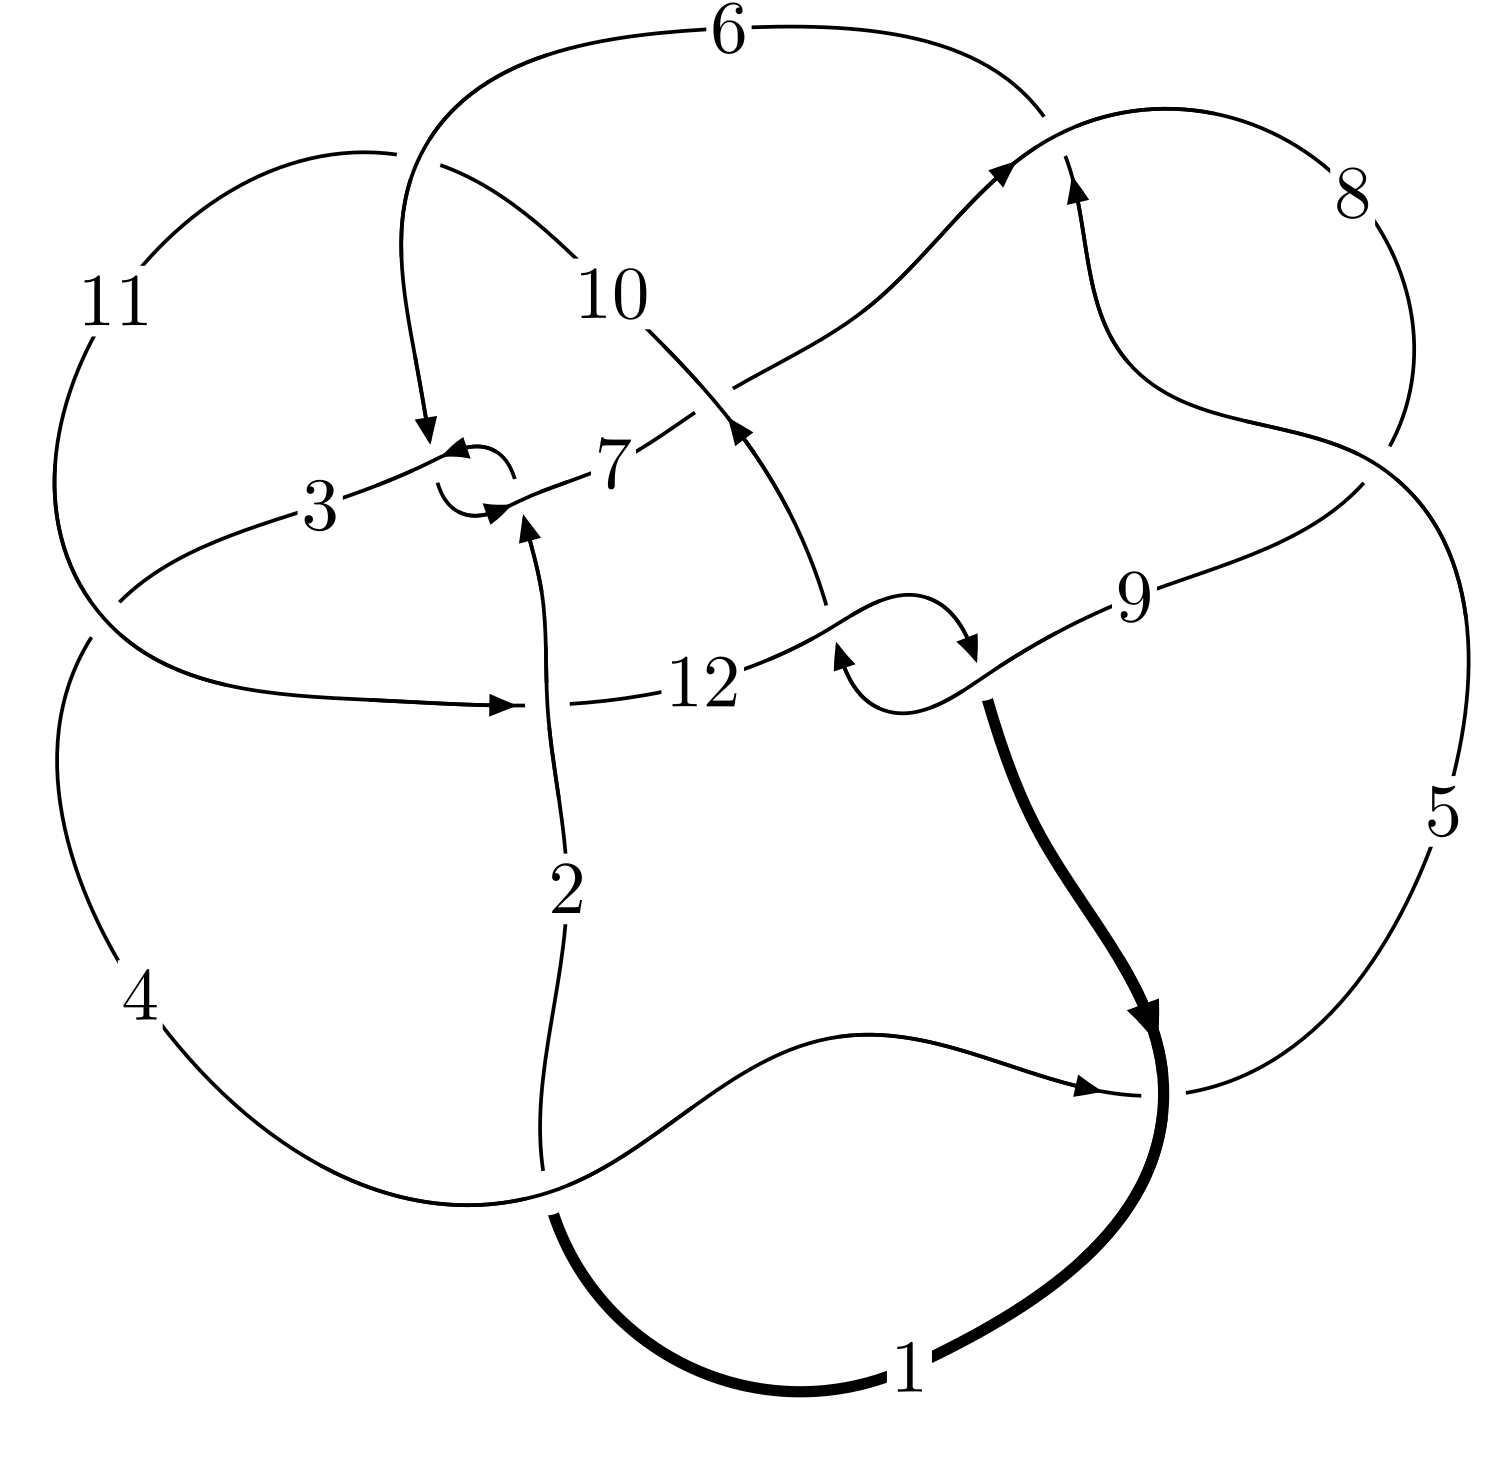
\includegraphics[width=112pt]{../../../GIT/diagram.site/Diagrams/png/1907_12a_1106.png}\\
\ \ \ A knot diagram\footnotemark}&
\allowdisplaybreaks
\textbf{Linearized knot diagam} \\
\cline{2-2}
 &
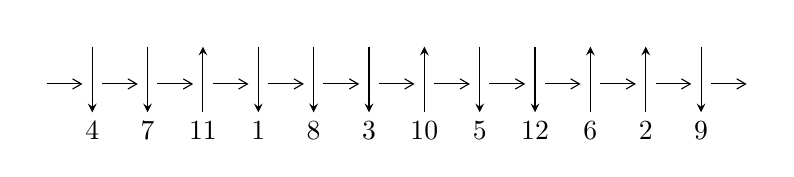
\begin{tikzpicture}[x=20pt, y=17pt]
	% nodes
	\node (C0) at (0, 0) {};
	\node (C1) at (1, 0) {};
	\node (C1U) at (1, +1) {};
	\node (C1D) at (1, -1) {4};

	\node (C2) at (2, 0) {};
	\node (C2U) at (2, +1) {};
	\node (C2D) at (2, -1) {7};

	\node (C3) at (3, 0) {};
	\node (C3U) at (3, +1) {};
	\node (C3D) at (3, -1) {11};

	\node (C4) at (4, 0) {};
	\node (C4U) at (4, +1) {};
	\node (C4D) at (4, -1) {1};

	\node (C5) at (5, 0) {};
	\node (C5U) at (5, +1) {};
	\node (C5D) at (5, -1) {8};

	\node (C6) at (6, 0) {};
	\node (C6U) at (6, +1) {};
	\node (C6D) at (6, -1) {3};

	\node (C7) at (7, 0) {};
	\node (C7U) at (7, +1) {};
	\node (C7D) at (7, -1) {10};

	\node (C8) at (8, 0) {};
	\node (C8U) at (8, +1) {};
	\node (C8D) at (8, -1) {5};

	\node (C9) at (9, 0) {};
	\node (C9U) at (9, +1) {};
	\node (C9D) at (9, -1) {12};

	\node (C10) at (10, 0) {};
	\node (C10U) at (10, +1) {};
	\node (C10D) at (10, -1) {6};

	\node (C11) at (11, 0) {};
	\node (C11U) at (11, +1) {};
	\node (C11D) at (11, -1) {2};

	\node (C12) at (12, 0) {};
	\node (C12U) at (12, +1) {};
	\node (C12D) at (12, -1) {9};
	\node (C13) at (13, 0) {};

	% arrows
	\draw[->,>={angle 60}]
	(C0) edge (C1) (C1) edge (C2) (C2) edge (C3) (C3) edge (C4) (C4) edge (C5) (C5) edge (C6) (C6) edge (C7) (C7) edge (C8) (C8) edge (C9) (C9) edge (C10) (C10) edge (C11) (C11) edge (C12) (C12) edge (C13) ;	\draw[->,>=stealth]
	(C1U) edge (C1D) (C2U) edge (C2D) (C3D) edge (C3U) (C4U) edge (C4D) (C5U) edge (C5D) (C6U) edge (C6D) (C7D) edge (C7U) (C8U) edge (C8D) (C9U) edge (C9D) (C10D) edge (C10U) (C11D) edge (C11U) (C12U) edge (C12D) ;
	\end{tikzpicture} \\
\hhline{~~} \\& 
\textbf{Solving Sequence} \\ \cline{2-2} 
 &
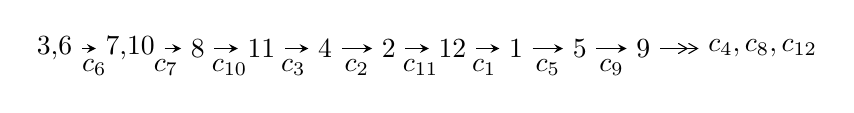
\begin{tikzpicture}[x=23pt, y=7pt]
	% node
	\node (A0) at (-1/8, 0) {3,6};
	\node (A1) at (17/16, 0) {7,10};
	\node (A2) at (17/8, 0) {8};
	\node (A3) at (25/8, 0) {11};
	\node (A4) at (33/8, 0) {4};
	\node (A5) at (41/8, 0) {2};
	\node (A6) at (49/8, 0) {12};
	\node (A7) at (57/8, 0) {1};
	\node (A8) at (65/8, 0) {5};
	\node (A9) at (73/8, 0) {9};
	\node (C1) at (1/2, -1) {$c_{6}$};
	\node (C2) at (13/8, -1) {$c_{7}$};
	\node (C3) at (21/8, -1) {$c_{10}$};
	\node (C4) at (29/8, -1) {$c_{3}$};
	\node (C5) at (37/8, -1) {$c_{2}$};
	\node (C6) at (45/8, -1) {$c_{11}$};
	\node (C7) at (53/8, -1) {$c_{1}$};
	\node (C8) at (61/8, -1) {$c_{5}$};
	\node (C9) at (69/8, -1) {$c_{9}$};
	\node (A10) at (11, 0) {$c_{4},c_{8},c_{12}$};

	% edge
	\draw[->,>=stealth]	
	(A0) edge (A1) (A1) edge (A2) (A2) edge (A3) (A3) edge (A4) (A4) edge (A5) (A5) edge (A6) (A6) edge (A7) (A7) edge (A8) (A8) edge (A9) ;
	\draw[->>,>={angle 60}]	
	(A9) edge (A10);
\end{tikzpicture} \\ 

\end{tabular} \\

\footnotetext{
The image of knot diagram is generated by the software ``\textbf{Draw programme}" developed by Andrew Bartholomew(\url{http://www.layer8.co.uk/maths/draw/index.htm\#Running-draw}), where we modified some parts for our purpose(\url{https://github.com/CATsTAILs/LinksPainter}).
}\phantom \\ \newline 
\centering \textbf{Ideals for irreducible components\footnotemark of $X_{\text{par}}$} 
 
\begin{align*}
I^u_{1}&=\langle 
-4.60339\times10^{20} u^{45}-6.13256\times10^{21} u^{44}+\cdots+3.13338\times10^{20} b-5.65347\times10^{22},\\
\phantom{I^u_{1}}&\phantom{= \langle  }-8.14927\times10^{21} u^{45}-9.80301\times10^{22} u^{44}+\cdots+4.07340\times10^{21} a-3.64681\times10^{23},\\
\phantom{I^u_{1}}&\phantom{= \langle  }u^{46}+13 u^{45}+\cdots+528 u+52\rangle \\
I^u_{2}&=\langle 
-2.52311\times10^{41} a u^{48}+4.74776\times10^{45} u^{48}+\cdots+1.26156\times10^{42} a-1.24713\times10^{46},\\
\phantom{I^u_{2}}&\phantom{= \langle  }-2.57277\times10^{43} a u^{48}-5.51496\times10^{43} u^{48}+\cdots-6.30524\times10^{44} a-2.26929\times10^{44},\\
\phantom{I^u_{2}}&\phantom{= \langle  }u^{49}-5 u^{48}+\cdots-24 u+5\rangle \\
I^u_{3}&=\langle 
39 u^{23}-272 u^{22}+\cdots+2 b+298,\;-227 u^{23}+1814 u^{22}+\cdots+4 a-104,\;u^{24}-8 u^{23}+\cdots-14 u+4\rangle \\
I^u_{4}&=\langle 
- u^8 a-2 u^8+\cdots- a+12,\;-2 u^8 a+4 u^8+\cdots-5 a+4,\\
\phantom{I^u_{4}}&\phantom{= \langle  }u^9+3 u^8+8 u^7+11 u^6+15 u^5+12 u^4+12 u^3+6 u^2+4 u+1\rangle \\
\\
\end{align*}
\raggedright * 4 irreducible components of $\dim_{\mathbb{C}}=0$, with total 186 representations.\\
\footnotetext{All coefficients of polynomials are rational numbers. But the coefficients are sometimes approximated in decimal forms when there is not enough margin.}
\newpage
\renewcommand{\arraystretch}{1}
\centering \section*{I. $I^u_{1}= \langle -4.60\times10^{20} u^{45}-6.13\times10^{21} u^{44}+\cdots+3.13\times10^{20} b-5.65\times10^{22},\;-8.15\times10^{21} u^{45}-9.80\times10^{22} u^{44}+\cdots+4.07\times10^{21} a-3.65\times10^{23},\;u^{46}+13 u^{45}+\cdots+528 u+52 \rangle$}
\flushleft \textbf{(i) Arc colorings}\\
\begin{tabular}{m{7pt} m{180pt} m{7pt} m{180pt} }
\flushright $a_{3}=$&$\begin{pmatrix}0\\u\end{pmatrix}$ \\
\flushright $a_{6}=$&$\begin{pmatrix}1\\0\end{pmatrix}$ \\
\flushright $a_{7}=$&$\begin{pmatrix}1\\u^2\end{pmatrix}$ \\
\flushright $a_{10}=$&$\begin{pmatrix}2.00061 u^{45}+24.0659 u^{44}+\cdots+818.429 u+89.5274\\1.46914 u^{45}+19.5717 u^{44}+\cdots+1562.07 u+180.427\end{pmatrix}$ \\
\flushright $a_{8}=$&$\begin{pmatrix}-4.00772 u^{45}-51.8972 u^{44}+\cdots-2075.81 u-216.751\\-1.86528 u^{45}-22.5866 u^{44}+\cdots-2577.80 u-305.396\end{pmatrix}$ \\
\flushright $a_{11}=$&$\begin{pmatrix}3.46975 u^{45}+43.6376 u^{44}+\cdots+2380.50 u+269.954\\1.46914 u^{45}+19.5717 u^{44}+\cdots+1562.07 u+180.427\end{pmatrix}$ \\
\flushright $a_{4}=$&$\begin{pmatrix}-6.58633 u^{45}-80.4182 u^{44}+\cdots-5130.89 u-595.022\\-5.20411 u^{45}-63.1627 u^{44}+\cdots-2881.56 u-342.489\end{pmatrix}$ \\
\flushright $a_{2}=$&$\begin{pmatrix}u\\u^3+u\end{pmatrix}$ \\
\flushright $a_{12}=$&$\begin{pmatrix}2.09825 u^{45}+27.7764 u^{44}+\cdots+2050.58 u+229.638\\-0.444574 u^{45}-6.01583 u^{44}+\cdots+264.191 u+37.7574\end{pmatrix}$ \\
\flushright $a_{1}=$&$\begin{pmatrix}-9.79082 u^{45}-125.313 u^{44}+\cdots-5041.79 u-538.637\\-3.63013 u^{45}-47.9190 u^{44}+\cdots-5309.39 u-606.117\end{pmatrix}$ \\
\flushright $a_{5}=$&$\begin{pmatrix}5.55453 u^{45}+70.1876 u^{44}+\cdots+3099.66 u+331.686\\-2.63800 u^{45}-30.8944 u^{44}+\cdots-683.228 u-70.7210\end{pmatrix}$ \\
\flushright $a_{9}=$&$\begin{pmatrix}8.06685 u^{45}+102.106 u^{44}+\cdots+5565.75 u+618.858\\1.02710 u^{45}+14.1539 u^{44}+\cdots+2593.21 u+305.374\end{pmatrix}$\\&\end{tabular}
\flushleft \textbf{(ii) Obstruction class $= -1$}\\~\\
\flushleft \textbf{(iii) Cusp Shapes $= -\frac{1739513054631728078213}{156669125128683693623} u^{45}-\frac{19720374536040326128317}{156669125128683693623} u^{44}+\cdots+\frac{65726012224390325344578}{156669125128683693623} u+\frac{6323936967181692502404}{156669125128683693623}$}\\~\\
\newpage\renewcommand{\arraystretch}{1}
\flushleft \textbf{(iv) u-Polynomials at the component}\newline \\
\begin{tabular}{m{50pt}|m{274pt}}
Crossings & \hspace{64pt}u-Polynomials at each crossing \\
\hline $$\begin{aligned}c_{1},c_{4},c_{5}\\c_{8}\end{aligned}$$&$\begin{aligned}
&u^{46}- u^{45}+\cdots+4 u+1
\end{aligned}$\\
\hline $$\begin{aligned}c_{2},c_{6}\end{aligned}$$&$\begin{aligned}
&u^{46}+13 u^{45}+\cdots+528 u+52
\end{aligned}$\\
\hline $$\begin{aligned}c_{3},c_{10}\end{aligned}$$&$\begin{aligned}
&u^{46}- u^{45}+\cdots- u+1
\end{aligned}$\\
\hline $$\begin{aligned}c_{7},c_{11}\end{aligned}$$&$\begin{aligned}
&u^{46}+3 u^{45}+\cdots+44 u+19
\end{aligned}$\\
\hline $$\begin{aligned}c_{9},c_{12}\end{aligned}$$&$\begin{aligned}
&u^{46}-16 u^{45}+\cdots-4284 u+356
\end{aligned}$\\
\hline
\end{tabular}\\~\\
\newpage\renewcommand{\arraystretch}{1}
\flushleft \textbf{(v) Riley Polynomials at the component}\newline \\
\begin{tabular}{m{50pt}|m{274pt}}
Crossings & \hspace{64pt}Riley Polynomials at each crossing \\
\hline $$\begin{aligned}c_{1},c_{4},c_{5}\\c_{8}\end{aligned}$$&$\begin{aligned}
&y^{46}+51 y^{45}+\cdots+46 y+1
\end{aligned}$\\
\hline $$\begin{aligned}c_{2},c_{6}\end{aligned}$$&$\begin{aligned}
&y^{46}+25 y^{45}+\cdots+38416 y+2704
\end{aligned}$\\
\hline $$\begin{aligned}c_{3},c_{10}\end{aligned}$$&$\begin{aligned}
&y^{46}-31 y^{45}+\cdots-37 y+1
\end{aligned}$\\
\hline $$\begin{aligned}c_{7},c_{11}\end{aligned}$$&$\begin{aligned}
&y^{46}-11 y^{45}+\cdots-74 y+361
\end{aligned}$\\
\hline $$\begin{aligned}c_{9},c_{12}\end{aligned}$$&$\begin{aligned}
&y^{46}+28 y^{45}+\cdots+6976 y+126736
\end{aligned}$\\
\hline
\end{tabular}\\~\\
\newpage\flushleft \textbf{(vi) Complex Volumes and Cusp Shapes}
$$\begin{array}{c|c|c}  
\text{Solutions to }I^u_{1}& \I (\text{vol} + \sqrt{-1}CS) & \text{Cusp shape}\\
 \hline 
\begin{aligned}
u &= \phantom{-}0.807598 + 0.595089 I \\
a &= \phantom{-}0.145048 - 0.406650 I \\
b &= -0.139471 + 0.179847 I\end{aligned}
 & \phantom{-}2.14007 - 2.35023 I & \phantom{-0.000000 } 0 \\ \hline\begin{aligned}
u &= \phantom{-}0.807598 - 0.595089 I \\
a &= \phantom{-}0.145048 + 0.406650 I \\
b &= -0.139471 - 0.179847 I\end{aligned}
 & \phantom{-}2.14007 + 2.35023 I & \phantom{-0.000000 } 0 \\ \hline\begin{aligned}
u &= \phantom{-}0.231176 + 0.989385 I \\
a &= -1.43994 + 0.06005 I \\
b &= \phantom{-}0.753112 + 0.540664 I\end{aligned}
 & \phantom{-}1.24241 - 3.60901 I & \phantom{-0.000000 } 0 \\ \hline\begin{aligned}
u &= \phantom{-}0.231176 - 0.989385 I \\
a &= -1.43994 - 0.06005 I \\
b &= \phantom{-}0.753112 - 0.540664 I\end{aligned}
 & \phantom{-}1.24241 + 3.60901 I & \phantom{-0.000000 } 0 \\ \hline\begin{aligned}
u &= -0.958272 + 0.171846 I \\
a &= -0.139418 - 0.213175 I \\
b &= -1.218050 + 0.694851 I\end{aligned}
 & \phantom{-}6.01083 - 6.65776 I & \phantom{-0.000000 } 0 \\ \hline\begin{aligned}
u &= -0.958272 - 0.171846 I \\
a &= -0.139418 + 0.213175 I \\
b &= -1.218050 - 0.694851 I\end{aligned}
 & \phantom{-}6.01083 + 6.65776 I & \phantom{-0.000000 } 0 \\ \hline\begin{aligned}
u &= -0.133424 + 0.931610 I \\
a &= -1.83866 - 0.63682 I \\
b &= \phantom{-}0.48794 + 1.35404 I\end{aligned}
 & \phantom{-}1.87823 + 0.64171 I & \phantom{-}7.20970 + 0. I\phantom{ +0.000000I} \\ \hline\begin{aligned}
u &= -0.133424 - 0.931610 I \\
a &= -1.83866 + 0.63682 I \\
b &= \phantom{-}0.48794 - 1.35404 I\end{aligned}
 & \phantom{-}1.87823 - 0.64171 I & \phantom{-}7.20970 + 0. I\phantom{ +0.000000I} \\ \hline\begin{aligned}
u &= -0.850515 + 0.368554 I \\
a &= \phantom{-}0.199127 + 0.211355 I \\
b &= \phantom{-}0.481513 - 0.475580 I\end{aligned}
 & -1.68076 + 0.65406 I & -4.00000 + 0. I\phantom{ +0.000000I} \\ \hline\begin{aligned}
u &= -0.850515 - 0.368554 I \\
a &= \phantom{-}0.199127 - 0.211355 I \\
b &= \phantom{-}0.481513 + 0.475580 I\end{aligned}
 & -1.68076 - 0.65406 I & -4.00000 + 0. I\phantom{ +0.000000I}\\
 \hline 
 \end{array}$$\newpage$$\begin{array}{c|c|c}  
\text{Solutions to }I^u_{1}& \I (\text{vol} + \sqrt{-1}CS) & \text{Cusp shape}\\
 \hline 
\begin{aligned}
u &= \phantom{-}0.079950 + 1.109550 I \\
a &= \phantom{-}1.71790 - 0.71105 I \\
b &= -1.273120 - 0.404326 I\end{aligned}
 & \phantom{-}12.79600 + 1.32693 I & \phantom{-0.000000 } 0 \\ \hline\begin{aligned}
u &= \phantom{-}0.079950 - 1.109550 I \\
a &= \phantom{-}1.71790 + 0.71105 I \\
b &= -1.273120 + 0.404326 I\end{aligned}
 & \phantom{-}12.79600 - 1.32693 I & \phantom{-0.000000 } 0 \\ \hline\begin{aligned}
u &= -0.123378 + 0.876834 I \\
a &= -1.62741 + 1.21693 I \\
b &= \phantom{-}1.39351 + 0.40523 I\end{aligned}
 & \phantom{-}11.46350 - 1.33067 I & \phantom{-}5.54801 + 0. I\phantom{ +0.000000I} \\ \hline\begin{aligned}
u &= -0.123378 - 0.876834 I \\
a &= -1.62741 - 1.21693 I \\
b &= \phantom{-}1.39351 - 0.40523 I\end{aligned}
 & \phantom{-}11.46350 + 1.33067 I & \phantom{-}5.54801 + 0. I\phantom{ +0.000000I} \\ \hline\begin{aligned}
u &= -1.136830 + 0.116641 I \\
a &= -0.090473 + 0.188791 I \\
b &= \phantom{-}1.154570 - 0.661441 I\end{aligned}
 & \phantom{-}10.9076 - 13.1169 I & \phantom{-0.000000 } 0 \\ \hline\begin{aligned}
u &= -1.136830 - 0.116641 I \\
a &= -0.090473 - 0.188791 I \\
b &= \phantom{-}1.154570 + 0.661441 I\end{aligned}
 & \phantom{-}10.9076 + 13.1169 I & \phantom{-0.000000 } 0 \\ \hline\begin{aligned}
u &= -1.177030 + 0.246057 I \\
a &= \phantom{-}0.100844 - 0.173825 I \\
b &= -0.760628 + 0.238675 I\end{aligned}
 & -0.28329 - 2.46940 I & \phantom{-0.000000 } 0 \\ \hline\begin{aligned}
u &= -1.177030 - 0.246057 I \\
a &= \phantom{-}0.100844 + 0.173825 I \\
b &= -0.760628 - 0.238675 I\end{aligned}
 & -0.28329 + 2.46940 I & \phantom{-0.000000 } 0 \\ \hline\begin{aligned}
u &= -0.553395 + 1.117580 I \\
a &= \phantom{-}0.674037 - 1.222200 I \\
b &= -1.40922 + 0.32528 I\end{aligned}
 & \phantom{-}13.4569 + 4.5178 I & \phantom{-0.000000 } 0 \\ \hline\begin{aligned}
u &= -0.553395 - 1.117580 I \\
a &= \phantom{-}0.674037 + 1.222200 I \\
b &= -1.40922 - 0.32528 I\end{aligned}
 & \phantom{-}13.4569 - 4.5178 I & \phantom{-0.000000 } 0\\
 \hline 
 \end{array}$$\newpage$$\begin{array}{c|c|c}  
\text{Solutions to }I^u_{1}& \I (\text{vol} + \sqrt{-1}CS) & \text{Cusp shape}\\
 \hline 
\begin{aligned}
u &= \phantom{-}0.587105 + 1.105440 I \\
a &= \phantom{-}0.597505 + 0.241208 I \\
b &= -0.272732 - 0.315437 I\end{aligned}
 & \phantom{-}7.07812 - 0.91875 I & \phantom{-0.000000 } 0 \\ \hline\begin{aligned}
u &= \phantom{-}0.587105 - 1.105440 I \\
a &= \phantom{-}0.597505 - 0.241208 I \\
b &= -0.272732 + 0.315437 I\end{aligned}
 & \phantom{-}7.07812 + 0.91875 I & \phantom{-0.000000 } 0 \\ \hline\begin{aligned}
u &= -0.225696 + 0.704958 I \\
a &= \phantom{-}1.345580 - 0.046479 I \\
b &= -0.425277 - 0.851426 I\end{aligned}
 & -0.34086 + 1.39531 I & -7.67124 - 3.20232 I \\ \hline\begin{aligned}
u &= -0.225696 - 0.704958 I \\
a &= \phantom{-}1.345580 + 0.046479 I \\
b &= -0.425277 + 0.851426 I\end{aligned}
 & -0.34086 - 1.39531 I & -7.67124 + 3.20232 I \\ \hline\begin{aligned}
u &= -0.410569 + 1.212210 I \\
a &= \phantom{-}2.01084 - 0.24207 I \\
b &= -1.52000 - 1.17808 I\end{aligned}
 & \phantom{-}14.4173 + 3.8759 I & \phantom{-0.000000 } 0 \\ \hline\begin{aligned}
u &= -0.410569 - 1.212210 I \\
a &= \phantom{-}2.01084 + 0.24207 I \\
b &= -1.52000 + 1.17808 I\end{aligned}
 & \phantom{-}14.4173 - 3.8759 I & \phantom{-0.000000 } 0 \\ \hline\begin{aligned}
u &= \phantom{-}1.114170 + 0.678095 I \\
a &= -0.373922 + 0.123021 I \\
b &= \phantom{-}0.230477 - 0.018824 I\end{aligned}
 & \phantom{-}5.21462 - 5.32991 I & \phantom{-0.000000 } 0 \\ \hline\begin{aligned}
u &= \phantom{-}1.114170 - 0.678095 I \\
a &= -0.373922 - 0.123021 I \\
b &= \phantom{-}0.230477 + 0.018824 I\end{aligned}
 & \phantom{-}5.21462 + 5.32991 I & \phantom{-0.000000 } 0 \\ \hline\begin{aligned}
u &= -0.677172 + 0.036174 I \\
a &= \phantom{-}0.490434 + 0.446612 I \\
b &= \phantom{-}1.163000 + 0.751547 I\end{aligned}
 & \phantom{-}10.79730 - 0.17282 I & \phantom{-}2.61634 - 1.42688 I \\ \hline\begin{aligned}
u &= -0.677172 - 0.036174 I \\
a &= \phantom{-}0.490434 - 0.446612 I \\
b &= \phantom{-}1.163000 - 0.751547 I\end{aligned}
 & \phantom{-}10.79730 + 0.17282 I & \phantom{-}2.61634 + 1.42688 I\\
 \hline 
 \end{array}$$\newpage$$\begin{array}{c|c|c}  
\text{Solutions to }I^u_{1}& \I (\text{vol} + \sqrt{-1}CS) & \text{Cusp shape}\\
 \hline 
\begin{aligned}
u &= -0.315606 + 1.283940 I \\
a &= -1.034810 + 0.862364 I \\
b &= \phantom{-}1.223300 + 0.044072 I\end{aligned}
 & \phantom{-}10.86770 - 2.33603 I & \phantom{-0.000000 } 0 \\ \hline\begin{aligned}
u &= -0.315606 - 1.283940 I \\
a &= -1.034810 - 0.862364 I \\
b &= \phantom{-}1.223300 - 0.044072 I\end{aligned}
 & \phantom{-}10.86770 + 2.33603 I & \phantom{-0.000000 } 0 \\ \hline\begin{aligned}
u &= -0.519948 + 1.222880 I \\
a &= \phantom{-}1.245960 - 0.257027 I \\
b &= -1.081520 - 0.697292 I\end{aligned}
 & \phantom{-}1.18366 + 4.44726 I & \phantom{-0.000000 } 0 \\ \hline\begin{aligned}
u &= -0.519948 - 1.222880 I \\
a &= \phantom{-}1.245960 + 0.257027 I \\
b &= -1.081520 + 0.697292 I\end{aligned}
 & \phantom{-}1.18366 - 4.44726 I & \phantom{-0.000000 } 0 \\ \hline\begin{aligned}
u &= -0.550737 + 1.253470 I \\
a &= -1.79269 + 0.41681 I \\
b &= \phantom{-}1.63311 + 0.95618 I\end{aligned}
 & \phantom{-}9.3517 + 12.1022 I & \phantom{-0.000000 } 0 \\ \hline\begin{aligned}
u &= -0.550737 - 1.253470 I \\
a &= -1.79269 - 0.41681 I \\
b &= \phantom{-}1.63311 - 0.95618 I\end{aligned}
 & \phantom{-}9.3517 - 12.1022 I & \phantom{-0.000000 } 0 \\ \hline\begin{aligned}
u &= -0.286358 + 1.351340 I \\
a &= -1.179040 + 0.177372 I \\
b &= \phantom{-}0.921389 + 0.559060 I\end{aligned}
 & \phantom{-}5.63593 + 2.22264 I & \phantom{-0.000000 } 0 \\ \hline\begin{aligned}
u &= -0.286358 - 1.351340 I \\
a &= -1.179040 - 0.177372 I \\
b &= \phantom{-}0.921389 - 0.559060 I\end{aligned}
 & \phantom{-}5.63593 - 2.22264 I & \phantom{-0.000000 } 0 \\ \hline\begin{aligned}
u &= -0.58550 + 1.33618 I \\
a &= \phantom{-}1.67084 - 0.31304 I \\
b &= -1.53069 - 0.89395 I\end{aligned}
 & \phantom{-}14.7508 + 19.1920 I & \phantom{-0.000000 } 0 \\ \hline\begin{aligned}
u &= -0.58550 - 1.33618 I \\
a &= \phantom{-}1.67084 + 0.31304 I \\
b &= -1.53069 + 0.89395 I\end{aligned}
 & \phantom{-}14.7508 - 19.1920 I & \phantom{-0.000000 } 0\\
 \hline 
 \end{array}$$\newpage$$\begin{array}{c|c|c}  
\text{Solutions to }I^u_{1}& \I (\text{vol} + \sqrt{-1}CS) & \text{Cusp shape}\\
 \hline 
\begin{aligned}
u &= -0.60654 + 1.32680 I \\
a &= -1.223140 + 0.285432 I \\
b &= \phantom{-}1.169600 + 0.620562 I\end{aligned}
 & \phantom{-}3.28252 + 8.78274 I & \phantom{-0.000000 } 0 \\ \hline\begin{aligned}
u &= -0.60654 - 1.32680 I \\
a &= -1.223140 - 0.285432 I \\
b &= \phantom{-}1.169600 - 0.620562 I\end{aligned}
 & \phantom{-}3.28252 - 8.78274 I & \phantom{-0.000000 } 0 \\ \hline\begin{aligned}
u &= -0.38466 + 1.48180 I \\
a &= \phantom{-}0.857403 - 0.686288 I \\
b &= -1.047490 + 0.028732 I\end{aligned}
 & \phantom{-}16.2619 - 7.4805 I & \phantom{-0.000000 } 0 \\ \hline\begin{aligned}
u &= -0.38466 - 1.48180 I \\
a &= \phantom{-}0.857403 + 0.686288 I \\
b &= -1.047490 - 0.028732 I\end{aligned}
 & \phantom{-}16.2619 + 7.4805 I & \phantom{-0.000000 } 0 \\ \hline\begin{aligned}
u &= \phantom{-}0.175636 + 0.397553 I \\
a &= \phantom{-}1.72245 - 0.09939 I \\
b &= -0.433330 - 0.421079 I\end{aligned}
 & -0.163355 + 1.344400 I & -0.935383 - 1.030188 I \\ \hline\begin{aligned}
u &= \phantom{-}0.175636 - 0.397553 I \\
a &= \phantom{-}1.72245 + 0.09939 I \\
b &= -0.433330 + 0.421079 I\end{aligned}
 & -0.163355 - 1.344400 I & -0.935383 + 1.030188 I\\
 \hline 
 \end{array}$$\newpage\newpage\renewcommand{\arraystretch}{1}
\centering \section*{II. $I^u_{2}= \langle -2.52\times10^{41} a u^{48}+4.75\times10^{45} u^{48}+\cdots+1.26\times10^{42} a-1.25\times10^{46},\;-2.57\times10^{43} a u^{48}-5.51\times10^{43} u^{48}+\cdots-6.31\times10^{44} a-2.27\times10^{44},\;u^{49}-5 u^{48}+\cdots-24 u+5 \rangle$}
\flushleft \textbf{(i) Arc colorings}\\
\begin{tabular}{m{7pt} m{180pt} m{7pt} m{180pt} }
\flushright $a_{3}=$&$\begin{pmatrix}0\\u\end{pmatrix}$ \\
\flushright $a_{6}=$&$\begin{pmatrix}1\\0\end{pmatrix}$ \\
\flushright $a_{7}=$&$\begin{pmatrix}1\\u^2\end{pmatrix}$ \\
\flushright $a_{10}=$&$\begin{pmatrix}a\\0.000388350 a u^{48}-7.30759 u^{48}+\cdots-0.00194175 a+19.1954\end{pmatrix}$ \\
\flushright $a_{8}=$&$\begin{pmatrix}0.558404 a u^{48}-4.16725 u^{48}+\cdots-21.6247 a-4.70757\\-0.798041 a u^{48}-0.836990 u^{48}+\cdots-14.9132 a+38.8839\end{pmatrix}$ \\
\flushright $a_{11}=$&$\begin{pmatrix}0.000388350 a u^{48}-7.30759 u^{48}+\cdots+0.998058 a+19.1954\\0.000388350 a u^{48}-7.30759 u^{48}+\cdots-0.00194175 a+19.1954\end{pmatrix}$ \\
\flushright $a_{4}=$&$\begin{pmatrix}7.30759 a u^{48}-8.39539 u^{48}+\cdots-19.1954 a-12.6628\\-7.06522 u^{48}+35.5339 u^{47}+\cdots-142.655 u+24.4019\end{pmatrix}$ \\
\flushright $a_{2}=$&$\begin{pmatrix}u\\u^3+u\end{pmatrix}$ \\
\flushright $a_{12}=$&$\begin{pmatrix}-4.28213 u^{48}+22.8488 u^{47}+\cdots+a+21.9874\\-0.000388350 a u^{48}-6.31628 u^{48}+\cdots+0.00194175 a+15.9948\end{pmatrix}$ \\
\flushright $a_{1}=$&$\begin{pmatrix}-4.17147 a u^{48}+5.85731 u^{48}+\cdots+29.7650 a-59.5141\\0.878342 a u^{48}+0.836990 u^{48}+\cdots+5.90205 a-37.8839\end{pmatrix}$ \\
\flushright $a_{5}=$&$\begin{pmatrix}-3.32947 a u^{48}-1.66919 u^{48}+\cdots+7.94493 a-43.2952\\0.897083 a u^{48}+2.34292 u^{48}+\cdots+16.2745 a-40.3382\end{pmatrix}$ \\
\flushright $a_{9}=$&$\begin{pmatrix}-3.75017 a u^{48}+3.58649 u^{48}+\cdots-10.6560 a-8.10556\\-0.917110 a u^{48}-1.49781 u^{48}+\cdots+12.6166 a+7.49436\end{pmatrix}$\\&\end{tabular}
\flushleft \textbf{(ii) Obstruction class $= -1$}\\~\\
\flushleft \textbf{(iii) Cusp Shapes $= -24.6678 u^{48}+121.656 u^{47}+\cdots-316.868 u-8.44978$}\\~\\
\newpage\renewcommand{\arraystretch}{1}
\flushleft \textbf{(iv) u-Polynomials at the component}\newline \\
\begin{tabular}{m{50pt}|m{274pt}}
Crossings & \hspace{64pt}u-Polynomials at each crossing \\
\hline $$\begin{aligned}c_{1},c_{4},c_{5}\\c_{8}\end{aligned}$$&$\begin{aligned}
&u^{98}-8 u^{97}+\cdots-1622 u+113
\end{aligned}$\\
\hline $$\begin{aligned}c_{2},c_{6}\end{aligned}$$&$\begin{aligned}
&(u^{49}-5 u^{48}+\cdots-24 u+5)^{2}
\end{aligned}$\\
\hline $$\begin{aligned}c_{3},c_{10}\end{aligned}$$&$\begin{aligned}
&u^{98}-2 u^{97}+\cdots-1030836 u+176389
\end{aligned}$\\
\hline $$\begin{aligned}c_{7},c_{11}\end{aligned}$$&$\begin{aligned}
&u^{98}+14 u^{97}+\cdots+155699 u+22103
\end{aligned}$\\
\hline $$\begin{aligned}c_{9},c_{12}\end{aligned}$$&$\begin{aligned}
&(u^{49}+12 u^{48}+\cdots+257 u+59)^{2}
\end{aligned}$\\
\hline
\end{tabular}\\~\\
\newpage\renewcommand{\arraystretch}{1}
\flushleft \textbf{(v) Riley Polynomials at the component}\newline \\
\begin{tabular}{m{50pt}|m{274pt}}
Crossings & \hspace{64pt}Riley Polynomials at each crossing \\
\hline $$\begin{aligned}c_{1},c_{4},c_{5}\\c_{8}\end{aligned}$$&$\begin{aligned}
&y^{98}+86 y^{97}+\cdots+162250 y+12769
\end{aligned}$\\
\hline $$\begin{aligned}c_{2},c_{6}\end{aligned}$$&$\begin{aligned}
&(y^{49}+33 y^{48}+\cdots-624 y-25)^{2}
\end{aligned}$\\
\hline $$\begin{aligned}c_{3},c_{10}\end{aligned}$$&$\begin{aligned}
&y^{98}-12 y^{97}+\cdots+591541541430 y+31113079321
\end{aligned}$\\
\hline $$\begin{aligned}c_{7},c_{11}\end{aligned}$$&$\begin{aligned}
&y^{98}-14 y^{97}+\cdots-3878773113 y+488542609
\end{aligned}$\\
\hline $$\begin{aligned}c_{9},c_{12}\end{aligned}$$&$\begin{aligned}
&(y^{49}+40 y^{48}+\cdots+20383 y-3481)^{2}
\end{aligned}$\\
\hline
\end{tabular}\\~\\
\newpage\flushleft \textbf{(vi) Complex Volumes and Cusp Shapes}
$$\begin{array}{c|c|c}  
\text{Solutions to }I^u_{2}& \I (\text{vol} + \sqrt{-1}CS) & \text{Cusp shape}\\
 \hline 
\begin{aligned}
u &= \phantom{-}0.957418 + 0.137707 I \\
a &= \phantom{-}0.286955 + 0.026555 I \\
b &= \phantom{-}0.770591 + 0.427917 I\end{aligned}
 & \phantom{-}0.78697 + 3.63609 I & -6.16185 - 3.13365 I \\ \hline\begin{aligned}
u &= \phantom{-}0.957418 + 0.137707 I \\
a &= \phantom{-}0.098397 + 0.256279 I \\
b &= -0.949930 - 0.580750 I\end{aligned}
 & \phantom{-}0.78697 + 3.63609 I & -6.16185 - 3.13365 I \\ \hline\begin{aligned}
u &= \phantom{-}0.957418 - 0.137707 I \\
a &= \phantom{-}0.286955 - 0.026555 I \\
b &= \phantom{-}0.770591 - 0.427917 I\end{aligned}
 & \phantom{-}0.78697 - 3.63609 I & -6.16185 + 3.13365 I \\ \hline\begin{aligned}
u &= \phantom{-}0.957418 - 0.137707 I \\
a &= \phantom{-}0.098397 - 0.256279 I \\
b &= -0.949930 + 0.580750 I\end{aligned}
 & \phantom{-}0.78697 - 3.63609 I & -6.16185 + 3.13365 I \\ \hline\begin{aligned}
u &= \phantom{-}0.264760 + 1.006070 I \\
a &= -0.52326 + 1.53050 I \\
b &= \phantom{-}0.02032 - 2.33382 I\end{aligned}
 & \phantom{-}10.39620 - 9.45799 I & \phantom{-0.000000 } 0 \\ \hline\begin{aligned}
u &= \phantom{-}0.264760 + 1.006070 I \\
a &= \phantom{-}2.83956 - 0.12888 I \\
b &= -0.675041 + 0.718691 I\end{aligned}
 & \phantom{-}10.39620 - 9.45799 I & \phantom{-0.000000 } 0 \\ \hline\begin{aligned}
u &= \phantom{-}0.264760 - 1.006070 I \\
a &= -0.52326 - 1.53050 I \\
b &= \phantom{-}0.02032 + 2.33382 I\end{aligned}
 & \phantom{-}10.39620 + 9.45799 I & \phantom{-0.000000 } 0 \\ \hline\begin{aligned}
u &= \phantom{-}0.264760 - 1.006070 I \\
a &= \phantom{-}2.83956 + 0.12888 I \\
b &= -0.675041 - 0.718691 I\end{aligned}
 & \phantom{-}10.39620 + 9.45799 I & \phantom{-0.000000 } 0 \\ \hline\begin{aligned}
u &= \phantom{-}0.226346 + 0.929253 I \\
a &= -0.148134 + 0.600625 I \\
b &= -0.020547 + 0.894164 I\end{aligned}
 & \phantom{-}0.67276 - 3.75122 I & -4.00000 + 10.38124 I \\ \hline\begin{aligned}
u &= \phantom{-}0.226346 + 0.929253 I \\
a &= -2.33048 - 0.06053 I \\
b &= \phantom{-}1.42722 - 0.18159 I\end{aligned}
 & \phantom{-}0.67276 - 3.75122 I & -4.00000 + 10.38124 I\\
 \hline 
 \end{array}$$\newpage$$\begin{array}{c|c|c}  
\text{Solutions to }I^u_{2}& \I (\text{vol} + \sqrt{-1}CS) & \text{Cusp shape}\\
 \hline 
\begin{aligned}
u &= \phantom{-}0.226346 - 0.929253 I \\
a &= -0.148134 - 0.600625 I \\
b &= -0.020547 - 0.894164 I\end{aligned}
 & \phantom{-}0.67276 + 3.75122 I & -4.00000 - 10.38124 I \\ \hline\begin{aligned}
u &= \phantom{-}0.226346 - 0.929253 I \\
a &= -2.33048 + 0.06053 I \\
b &= \phantom{-}1.42722 + 0.18159 I\end{aligned}
 & \phantom{-}0.67276 + 3.75122 I & -4.00000 - 10.38124 I \\ \hline\begin{aligned}
u &= -0.091513 + 0.935745 I \\
a &= -0.456898 - 0.674035 I \\
b &= -0.18764 + 1.53444 I\end{aligned}
 & \phantom{-}1.92899 + 0.49464 I & \phantom{-}3.10942 + 0. I\phantom{ +0.000000I} \\ \hline\begin{aligned}
u &= -0.091513 + 0.935745 I \\
a &= -2.38983 - 0.72163 I \\
b &= \phantom{-}0.746133 + 0.681858 I\end{aligned}
 & \phantom{-}1.92899 + 0.49464 I & \phantom{-}3.10942 + 0. I\phantom{ +0.000000I} \\ \hline\begin{aligned}
u &= -0.091513 - 0.935745 I \\
a &= -0.456898 + 0.674035 I \\
b &= -0.18764 - 1.53444 I\end{aligned}
 & \phantom{-}1.92899 - 0.49464 I & \phantom{-}3.10942 + 0. I\phantom{ +0.000000I} \\ \hline\begin{aligned}
u &= -0.091513 - 0.935745 I \\
a &= -2.38983 + 0.72163 I \\
b &= \phantom{-}0.746133 - 0.681858 I\end{aligned}
 & \phantom{-}1.92899 - 0.49464 I & \phantom{-}3.10942 + 0. I\phantom{ +0.000000I} \\ \hline\begin{aligned}
u &= -0.156773 + 1.055540 I \\
a &= -1.012630 + 0.946873 I \\
b &= \phantom{-}1.08233 - 1.74068 I\end{aligned}
 & \phantom{-}6.66499 + 3.79319 I & \phantom{-0.000000 } 0 \\ \hline\begin{aligned}
u &= -0.156773 + 1.055540 I \\
a &= \phantom{-}2.58947 + 0.96162 I \\
b &= -0.826969 - 0.198015 I\end{aligned}
 & \phantom{-}6.66499 + 3.79319 I & \phantom{-0.000000 } 0 \\ \hline\begin{aligned}
u &= -0.156773 - 1.055540 I \\
a &= -1.012630 - 0.946873 I \\
b &= \phantom{-}1.08233 + 1.74068 I\end{aligned}
 & \phantom{-}6.66499 - 3.79319 I & \phantom{-0.000000 } 0 \\ \hline\begin{aligned}
u &= -0.156773 - 1.055540 I \\
a &= \phantom{-}2.58947 - 0.96162 I \\
b &= -0.826969 + 0.198015 I\end{aligned}
 & \phantom{-}6.66499 - 3.79319 I & \phantom{-0.000000 } 0\\
 \hline 
 \end{array}$$\newpage$$\begin{array}{c|c|c}  
\text{Solutions to }I^u_{2}& \I (\text{vol} + \sqrt{-1}CS) & \text{Cusp shape}\\
 \hline 
\begin{aligned}
u &= -0.346619 + 1.023320 I \\
a &= \phantom{-}0.016055 - 0.908875 I \\
b &= -0.22570 + 1.48864 I\end{aligned}
 & \phantom{-}4.55239 + 5.49253 I & \phantom{-0.000000 } 0 \\ \hline\begin{aligned}
u &= -0.346619 + 1.023320 I \\
a &= -1.89262 - 0.17132 I \\
b &= \phantom{-}0.520618 + 0.415489 I\end{aligned}
 & \phantom{-}4.55239 + 5.49253 I & \phantom{-0.000000 } 0 \\ \hline\begin{aligned}
u &= -0.346619 - 1.023320 I \\
a &= \phantom{-}0.016055 + 0.908875 I \\
b &= -0.22570 - 1.48864 I\end{aligned}
 & \phantom{-}4.55239 - 5.49253 I & \phantom{-0.000000 } 0 \\ \hline\begin{aligned}
u &= -0.346619 - 1.023320 I \\
a &= -1.89262 + 0.17132 I \\
b &= \phantom{-}0.520618 - 0.415489 I\end{aligned}
 & \phantom{-}4.55239 - 5.49253 I & \phantom{-0.000000 } 0 \\ \hline\begin{aligned}
u &= \phantom{-}0.255872 + 0.810452 I \\
a &= -2.33454 - 0.40118 I \\
b &= \phantom{-}0.036356 - 1.193870 I\end{aligned}
 & \phantom{-}3.99300 - 1.28672 I & -2.49363 + 5.09640 I \\ \hline\begin{aligned}
u &= \phantom{-}0.255872 + 0.810452 I \\
a &= \phantom{-}2.03137 - 1.80698 I \\
b &= -0.70468 + 2.27070 I\end{aligned}
 & \phantom{-}3.99300 - 1.28672 I & -2.49363 + 5.09640 I \\ \hline\begin{aligned}
u &= \phantom{-}0.255872 - 0.810452 I \\
a &= -2.33454 + 0.40118 I \\
b &= \phantom{-}0.036356 + 1.193870 I\end{aligned}
 & \phantom{-}3.99300 + 1.28672 I & -2.49363 - 5.09640 I \\ \hline\begin{aligned}
u &= \phantom{-}0.255872 - 0.810452 I \\
a &= \phantom{-}2.03137 + 1.80698 I \\
b &= -0.70468 - 2.27070 I\end{aligned}
 & \phantom{-}3.99300 + 1.28672 I & -2.49363 - 5.09640 I \\ \hline\begin{aligned}
u &= \phantom{-}0.650362 + 0.441524 I \\
a &= \phantom{-}0.677266 + 1.068720 I \\
b &= -1.096870 + 0.194713 I\end{aligned}
 & \phantom{-}5.53096 - 2.47656 I & \phantom{-}1.49723 + 2.71117 I \\ \hline\begin{aligned}
u &= \phantom{-}0.650362 + 0.441524 I \\
a &= \phantom{-}0.184610 - 0.352276 I \\
b &= \phantom{-}0.830729 - 0.636420 I\end{aligned}
 & \phantom{-}5.53096 - 2.47656 I & \phantom{-}1.49723 + 2.71117 I\\
 \hline 
 \end{array}$$\newpage$$\begin{array}{c|c|c}  
\text{Solutions to }I^u_{2}& \I (\text{vol} + \sqrt{-1}CS) & \text{Cusp shape}\\
 \hline 
\begin{aligned}
u &= \phantom{-}0.650362 - 0.441524 I \\
a &= \phantom{-}0.677266 - 1.068720 I \\
b &= -1.096870 - 0.194713 I\end{aligned}
 & \phantom{-}5.53096 + 2.47656 I & \phantom{-}1.49723 - 2.71117 I \\ \hline\begin{aligned}
u &= \phantom{-}0.650362 - 0.441524 I \\
a &= \phantom{-}0.184610 + 0.352276 I \\
b &= \phantom{-}0.830729 + 0.636420 I\end{aligned}
 & \phantom{-}5.53096 + 2.47656 I & \phantom{-}1.49723 - 2.71117 I \\ \hline\begin{aligned}
u &= \phantom{-}1.217590 + 0.050320 I \\
a &= -0.380129 - 0.100856 I \\
b &= \phantom{-}0.987499 + 0.498459 I\end{aligned}
 & \phantom{-}3.96783 + 6.46429 I & \phantom{-0.000000 } 0 \\ \hline\begin{aligned}
u &= \phantom{-}1.217590 + 0.050320 I \\
a &= -0.107019 + 0.139455 I \\
b &= -0.719519 - 0.514679 I\end{aligned}
 & \phantom{-}3.96783 + 6.46429 I & \phantom{-0.000000 } 0 \\ \hline\begin{aligned}
u &= \phantom{-}1.217590 - 0.050320 I \\
a &= -0.380129 + 0.100856 I \\
b &= \phantom{-}0.987499 - 0.498459 I\end{aligned}
 & \phantom{-}3.96783 - 6.46429 I & \phantom{-0.000000 } 0 \\ \hline\begin{aligned}
u &= \phantom{-}1.217590 - 0.050320 I \\
a &= -0.107019 - 0.139455 I \\
b &= -0.719519 + 0.514679 I\end{aligned}
 & \phantom{-}3.96783 - 6.46429 I & \phantom{-0.000000 } 0 \\ \hline\begin{aligned}
u &= -0.943010 + 0.818382 I \\
a &= -1.130180 + 0.715066 I \\
b &= \phantom{-}1.347900 - 0.119643 I\end{aligned}
 & \phantom{-}8.64456 + 5.11693 I & \phantom{-0.000000 } 0 \\ \hline\begin{aligned}
u &= -0.943010 + 0.818382 I \\
a &= \phantom{-}0.185523 + 0.251875 I \\
b &= \phantom{-}0.692592 + 0.383315 I\end{aligned}
 & \phantom{-}8.64456 + 5.11693 I & \phantom{-0.000000 } 0 \\ \hline\begin{aligned}
u &= -0.943010 - 0.818382 I \\
a &= -1.130180 - 0.715066 I \\
b &= \phantom{-}1.347900 + 0.119643 I\end{aligned}
 & \phantom{-}8.64456 - 5.11693 I & \phantom{-0.000000 } 0 \\ \hline\begin{aligned}
u &= -0.943010 - 0.818382 I \\
a &= \phantom{-}0.185523 - 0.251875 I \\
b &= \phantom{-}0.692592 - 0.383315 I\end{aligned}
 & \phantom{-}8.64456 - 5.11693 I & \phantom{-0.000000 } 0\\
 \hline 
 \end{array}$$\newpage$$\begin{array}{c|c|c}  
\text{Solutions to }I^u_{2}& \I (\text{vol} + \sqrt{-1}CS) & \text{Cusp shape}\\
 \hline 
\begin{aligned}
u &= -0.662579 + 0.318199 I \\
a &= -1.42153 + 0.15838 I \\
b &= \phantom{-}0.494020 + 0.798046 I\end{aligned}
 & \phantom{-}2.47935 - 1.74491 I & -2.56195 + 1.08924 I \\ \hline\begin{aligned}
u &= -0.662579 + 0.318199 I \\
a &= \phantom{-}0.446052 + 0.340850 I \\
b &= -0.310211 + 0.928842 I\end{aligned}
 & \phantom{-}2.47935 - 1.74491 I & -2.56195 + 1.08924 I \\ \hline\begin{aligned}
u &= -0.662579 - 0.318199 I \\
a &= -1.42153 - 0.15838 I \\
b &= \phantom{-}0.494020 - 0.798046 I\end{aligned}
 & \phantom{-}2.47935 + 1.74491 I & -2.56195 - 1.08924 I \\ \hline\begin{aligned}
u &= -0.662579 - 0.318199 I \\
a &= \phantom{-}0.446052 - 0.340850 I \\
b &= -0.310211 - 0.928842 I\end{aligned}
 & \phantom{-}2.47935 + 1.74491 I & -2.56195 - 1.08924 I \\ \hline\begin{aligned}
u &= -0.719602\phantom{ +0.000000I} \\
a &= -0.388671 + 1.087390 I \\
b &= -0.997469 - 0.455040 I\end{aligned}
 & \phantom{-}5.21368\phantom{ +0.000000I} & -1.16360\phantom{ +0.000000I} \\ \hline\begin{aligned}
u &= -0.719602\phantom{ +0.000000I} \\
a &= -0.388671 - 1.087390 I \\
b &= -0.997469 + 0.455040 I\end{aligned}
 & \phantom{-}5.21368\phantom{ +0.000000I} & -1.16360\phantom{ +0.000000I} \\ \hline\begin{aligned}
u &= \phantom{-}0.329381 + 1.249470 I \\
a &= -1.42789 - 0.56714 I \\
b &= \phantom{-}1.009110 - 0.770169 I\end{aligned}
 & \phantom{-}10.11660 - 5.76726 I & \phantom{-0.000000 } 0 \\ \hline\begin{aligned}
u &= \phantom{-}0.329381 + 1.249470 I \\
a &= \phantom{-}1.91025 - 0.05665 I \\
b &= -1.53298 + 0.96374 I\end{aligned}
 & \phantom{-}10.11660 - 5.76726 I & \phantom{-0.000000 } 0 \\ \hline\begin{aligned}
u &= \phantom{-}0.329381 - 1.249470 I \\
a &= -1.42789 + 0.56714 I \\
b &= \phantom{-}1.009110 + 0.770169 I\end{aligned}
 & \phantom{-}10.11660 + 5.76726 I & \phantom{-0.000000 } 0 \\ \hline\begin{aligned}
u &= \phantom{-}0.329381 - 1.249470 I \\
a &= \phantom{-}1.91025 + 0.05665 I \\
b &= -1.53298 - 0.96374 I\end{aligned}
 & \phantom{-}10.11660 + 5.76726 I & \phantom{-0.000000 } 0\\
 \hline 
 \end{array}$$\newpage$$\begin{array}{c|c|c}  
\text{Solutions to }I^u_{2}& \I (\text{vol} + \sqrt{-1}CS) & \text{Cusp shape}\\
 \hline 
\begin{aligned}
u &= \phantom{-}0.396490 + 1.239700 I \\
a &= -0.873184 - 0.814822 I \\
b &= \phantom{-}0.874312 - 0.185924 I\end{aligned}
 & \phantom{-}5.25338 - 0.75552 I & \phantom{-0.000000 } 0 \\ \hline\begin{aligned}
u &= \phantom{-}0.396490 + 1.239700 I \\
a &= \phantom{-}1.172500 + 0.287941 I \\
b &= -1.241080 + 0.395387 I\end{aligned}
 & \phantom{-}5.25338 - 0.75552 I & \phantom{-0.000000 } 0 \\ \hline\begin{aligned}
u &= \phantom{-}0.396490 - 1.239700 I \\
a &= -0.873184 + 0.814822 I \\
b &= \phantom{-}0.874312 + 0.185924 I\end{aligned}
 & \phantom{-}5.25338 + 0.75552 I & \phantom{-0.000000 } 0 \\ \hline\begin{aligned}
u &= \phantom{-}0.396490 - 1.239700 I \\
a &= \phantom{-}1.172500 - 0.287941 I \\
b &= -1.241080 - 0.395387 I\end{aligned}
 & \phantom{-}5.25338 + 0.75552 I & \phantom{-0.000000 } 0 \\ \hline\begin{aligned}
u &= -0.224605 + 0.658535 I \\
a &= \phantom{-}1.037960 + 0.472207 I \\
b &= -0.341084 - 1.075920 I\end{aligned}
 & -0.38164 + 1.40636 I & -7.90709 - 4.60491 I \\ \hline\begin{aligned}
u &= -0.224605 + 0.658535 I \\
a &= \phantom{-}1.54635 - 0.36863 I \\
b &= -0.241044 - 0.594512 I\end{aligned}
 & -0.38164 + 1.40636 I & -7.90709 - 4.60491 I \\ \hline\begin{aligned}
u &= -0.224605 - 0.658535 I \\
a &= \phantom{-}1.037960 - 0.472207 I \\
b &= -0.341084 + 1.075920 I\end{aligned}
 & -0.38164 - 1.40636 I & -7.90709 + 4.60491 I \\ \hline\begin{aligned}
u &= -0.224605 - 0.658535 I \\
a &= \phantom{-}1.54635 + 0.36863 I \\
b &= -0.241044 + 0.594512 I\end{aligned}
 & -0.38164 - 1.40636 I & -7.90709 + 4.60491 I \\ \hline\begin{aligned}
u &= -0.563956 + 1.217970 I \\
a &= -0.407390 + 0.754967 I \\
b &= \phantom{-}0.727020 + 0.391576 I\end{aligned}
 & \phantom{-}8.40264 + 4.63276 I & \phantom{-0.000000 } 0 \\ \hline\begin{aligned}
u &= -0.563956 + 1.217970 I \\
a &= -1.61386 + 0.35681 I \\
b &= \phantom{-}1.57671 + 0.25730 I\end{aligned}
 & \phantom{-}8.40264 + 4.63276 I & \phantom{-0.000000 } 0\\
 \hline 
 \end{array}$$\newpage$$\begin{array}{c|c|c}  
\text{Solutions to }I^u_{2}& \I (\text{vol} + \sqrt{-1}CS) & \text{Cusp shape}\\
 \hline 
\begin{aligned}
u &= -0.563956 - 1.217970 I \\
a &= -0.407390 - 0.754967 I \\
b &= \phantom{-}0.727020 - 0.391576 I\end{aligned}
 & \phantom{-}8.40264 - 4.63276 I & \phantom{-0.000000 } 0 \\ \hline\begin{aligned}
u &= -0.563956 - 1.217970 I \\
a &= -1.61386 - 0.35681 I \\
b &= \phantom{-}1.57671 - 0.25730 I\end{aligned}
 & \phantom{-}8.40264 - 4.63276 I & \phantom{-0.000000 } 0 \\ \hline\begin{aligned}
u &= -0.253681 + 1.320130 I \\
a &= \phantom{-}1.20869 - 1.20917 I \\
b &= -0.783841 - 0.186625 I\end{aligned}
 & \phantom{-}14.9725 + 8.1096 I & \phantom{-0.000000 } 0 \\ \hline\begin{aligned}
u &= -0.253681 + 1.320130 I \\
a &= \phantom{-}1.76114 + 0.31613 I \\
b &= -1.73484 - 0.91494 I\end{aligned}
 & \phantom{-}14.9725 + 8.1096 I & \phantom{-0.000000 } 0 \\ \hline\begin{aligned}
u &= -0.253681 - 1.320130 I \\
a &= \phantom{-}1.20869 + 1.20917 I \\
b &= -0.783841 + 0.186625 I\end{aligned}
 & \phantom{-}14.9725 - 8.1096 I & \phantom{-0.000000 } 0 \\ \hline\begin{aligned}
u &= -0.253681 - 1.320130 I \\
a &= \phantom{-}1.76114 - 0.31613 I \\
b &= -1.73484 + 0.91494 I\end{aligned}
 & \phantom{-}14.9725 - 8.1096 I & \phantom{-0.000000 } 0 \\ \hline\begin{aligned}
u &= \phantom{-}0.008742 + 0.639353 I \\
a &= -0.147556 - 1.227300 I \\
b &= \phantom{-}0.719465 - 0.763198 I\end{aligned}
 & \phantom{-}5.23017 - 2.51958 I & \phantom{-}1.241083 - 0.357010 I \\ \hline\begin{aligned}
u &= \phantom{-}0.008742 + 0.639353 I \\
a &= \phantom{-}2.45573 + 1.48966 I \\
b &= -1.277630 - 0.348252 I\end{aligned}
 & \phantom{-}5.23017 - 2.51958 I & \phantom{-}1.241083 - 0.357010 I \\ \hline\begin{aligned}
u &= \phantom{-}0.008742 - 0.639353 I \\
a &= -0.147556 + 1.227300 I \\
b &= \phantom{-}0.719465 + 0.763198 I\end{aligned}
 & \phantom{-}5.23017 + 2.51958 I & \phantom{-}1.241083 + 0.357010 I \\ \hline\begin{aligned}
u &= \phantom{-}0.008742 - 0.639353 I \\
a &= \phantom{-}2.45573 - 1.48966 I \\
b &= -1.277630 + 0.348252 I\end{aligned}
 & \phantom{-}5.23017 + 2.51958 I & \phantom{-}1.241083 + 0.357010 I\\
 \hline 
 \end{array}$$\newpage$$\begin{array}{c|c|c}  
\text{Solutions to }I^u_{2}& \I (\text{vol} + \sqrt{-1}CS) & \text{Cusp shape}\\
 \hline 
\begin{aligned}
u &= \phantom{-}0.531201 + 1.269820 I \\
a &= \phantom{-}1.337790 + 0.287032 I \\
b &= -1.21857 + 0.88759 I\end{aligned}
 & \phantom{-}4.30856 - 9.00359 I & \phantom{-0.000000 } 0 \\ \hline\begin{aligned}
u &= \phantom{-}0.531201 + 1.269820 I \\
a &= -1.68147 - 0.29022 I \\
b &= \phantom{-}1.42823 - 0.77535 I\end{aligned}
 & \phantom{-}4.30856 - 9.00359 I & \phantom{-0.000000 } 0 \\ \hline\begin{aligned}
u &= \phantom{-}0.531201 - 1.269820 I \\
a &= \phantom{-}1.337790 - 0.287032 I \\
b &= -1.21857 - 0.88759 I\end{aligned}
 & \phantom{-}4.30856 + 9.00359 I & \phantom{-0.000000 } 0 \\ \hline\begin{aligned}
u &= \phantom{-}0.531201 - 1.269820 I \\
a &= -1.68147 + 0.29022 I \\
b &= \phantom{-}1.42823 + 0.77535 I\end{aligned}
 & \phantom{-}4.30856 + 9.00359 I & \phantom{-0.000000 } 0 \\ \hline\begin{aligned}
u &= \phantom{-}0.324351 + 0.493941 I \\
a &= \phantom{-}0.515496 + 1.077260 I \\
b &= \phantom{-}0.647626 + 1.092120 I\end{aligned}
 & \phantom{-}8.96981 + 6.76225 I & -1.16496 - 1.32686 I \\ \hline\begin{aligned}
u &= \phantom{-}0.324351 + 0.493941 I \\
a &= -2.84073 + 1.17981 I \\
b &= \phantom{-}0.69428 - 1.27815 I\end{aligned}
 & \phantom{-}8.96981 + 6.76225 I & -1.16496 - 1.32686 I \\ \hline\begin{aligned}
u &= \phantom{-}0.324351 - 0.493941 I \\
a &= \phantom{-}0.515496 - 1.077260 I \\
b &= \phantom{-}0.647626 - 1.092120 I\end{aligned}
 & \phantom{-}8.96981 - 6.76225 I & -1.16496 + 1.32686 I \\ \hline\begin{aligned}
u &= \phantom{-}0.324351 - 0.493941 I \\
a &= -2.84073 - 1.17981 I \\
b &= \phantom{-}0.69428 + 1.27815 I\end{aligned}
 & \phantom{-}8.96981 - 6.76225 I & -1.16496 + 1.32686 I \\ \hline\begin{aligned}
u &= \phantom{-}0.72262 + 1.25115 I \\
a &= -1.029400 - 0.615681 I \\
b &= \phantom{-}1.240690 + 0.008012 I\end{aligned}
 & \phantom{-}7.38957 - 3.44269 I & \phantom{-0.000000 } 0 \\ \hline\begin{aligned}
u &= \phantom{-}0.72262 + 1.25115 I \\
a &= \phantom{-}0.478696 + 0.566053 I \\
b &= -0.912969 + 0.174762 I\end{aligned}
 & \phantom{-}7.38957 - 3.44269 I & \phantom{-0.000000 } 0\\
 \hline 
 \end{array}$$\newpage$$\begin{array}{c|c|c}  
\text{Solutions to }I^u_{2}& \I (\text{vol} + \sqrt{-1}CS) & \text{Cusp shape}\\
 \hline 
\begin{aligned}
u &= \phantom{-}0.72262 - 1.25115 I \\
a &= -1.029400 + 0.615681 I \\
b &= \phantom{-}1.240690 - 0.008012 I\end{aligned}
 & \phantom{-}7.38957 + 3.44269 I & \phantom{-0.000000 } 0 \\ \hline\begin{aligned}
u &= \phantom{-}0.72262 - 1.25115 I \\
a &= \phantom{-}0.478696 - 0.566053 I \\
b &= -0.912969 - 0.174762 I\end{aligned}
 & \phantom{-}7.38957 + 3.44269 I & \phantom{-0.000000 } 0 \\ \hline\begin{aligned}
u &= \phantom{-}0.155829 + 0.518115 I \\
a &= \phantom{-}1.000180 + 0.818212 I \\
b &= -0.664836 - 0.869546 I\end{aligned}
 & -0.29520 + 1.46947 I & -6.37279 - 1.95675 I \\ \hline\begin{aligned}
u &= \phantom{-}0.155829 + 0.518115 I \\
a &= \phantom{-}1.97184 - 0.54810 I \\
b &= -0.078854 - 0.165747 I\end{aligned}
 & -0.29520 + 1.46947 I & -6.37279 - 1.95675 I \\ \hline\begin{aligned}
u &= \phantom{-}0.155829 - 0.518115 I \\
a &= \phantom{-}1.000180 - 0.818212 I \\
b &= -0.664836 + 0.869546 I\end{aligned}
 & -0.29520 - 1.46947 I & -6.37279 + 1.95675 I \\ \hline\begin{aligned}
u &= \phantom{-}0.155829 - 0.518115 I \\
a &= \phantom{-}1.97184 + 0.54810 I \\
b &= -0.078854 + 0.165747 I\end{aligned}
 & -0.29520 - 1.46947 I & -6.37279 + 1.95675 I \\ \hline\begin{aligned}
u &= \phantom{-}0.57926 + 1.36321 I \\
a &= -1.312240 - 0.075466 I \\
b &= \phantom{-}1.23560 - 0.94753 I\end{aligned}
 & \phantom{-}8.1120 - 12.6788 I & \phantom{-0.000000 } 0 \\ \hline\begin{aligned}
u &= \phantom{-}0.57926 + 1.36321 I \\
a &= \phantom{-}1.61270 + 0.32089 I \\
b &= -1.35017 + 0.69705 I\end{aligned}
 & \phantom{-}8.1120 - 12.6788 I & \phantom{-0.000000 } 0 \\ \hline\begin{aligned}
u &= \phantom{-}0.57926 - 1.36321 I \\
a &= -1.312240 + 0.075466 I \\
b &= \phantom{-}1.23560 + 0.94753 I\end{aligned}
 & \phantom{-}8.1120 + 12.6788 I & \phantom{-0.000000 } 0 \\ \hline\begin{aligned}
u &= \phantom{-}0.57926 - 1.36321 I \\
a &= \phantom{-}1.61270 - 0.32089 I \\
b &= -1.35017 - 0.69705 I\end{aligned}
 & \phantom{-}8.1120 + 12.6788 I & \phantom{-0.000000 } 0\\
 \hline 
 \end{array}$$\newpage$$\begin{array}{c|c|c}  
\text{Solutions to }I^u_{2}& \I (\text{vol} + \sqrt{-1}CS) & \text{Cusp shape}\\
 \hline 
\begin{aligned}
u &= \phantom{-}0.27071 + 1.54654 I \\
a &= -0.733979 + 0.068037 I \\
b &= \phantom{-}0.853269 - 0.629295 I\end{aligned}
 & \phantom{-}9.84990 + 0.22502 I & \phantom{-0.000000 } 0 \\ \hline\begin{aligned}
u &= \phantom{-}0.27071 + 1.54654 I \\
a &= \phantom{-}1.201400 + 0.636983 I \\
b &= -0.900300 - 0.032549 I\end{aligned}
 & \phantom{-}9.84990 + 0.22502 I & \phantom{-0.000000 } 0 \\ \hline\begin{aligned}
u &= \phantom{-}0.27071 - 1.54654 I \\
a &= -0.733979 - 0.068037 I \\
b &= \phantom{-}0.853269 + 0.629295 I\end{aligned}
 & \phantom{-}9.84990 - 0.22502 I & \phantom{-0.000000 } 0 \\ \hline\begin{aligned}
u &= \phantom{-}0.27071 - 1.54654 I \\
a &= \phantom{-}1.201400 - 0.636983 I \\
b &= -0.900300 + 0.032549 I\end{aligned}
 & \phantom{-}9.84990 - 0.22502 I & \phantom{-0.000000 } 0 \\ \hline\begin{aligned}
u &= -0.78839 + 1.49937 I \\
a &= \phantom{-}1.379970 - 0.308325 I \\
b &= -1.283850 - 0.199748 I\end{aligned}
 & \phantom{-}10.60110 + 2.92501 I & \phantom{-0.000000 } 0 \\ \hline\begin{aligned}
u &= -0.78839 + 1.49937 I \\
a &= \phantom{-}0.437662 - 0.180997 I \\
b &= -0.686011 - 0.544678 I\end{aligned}
 & \phantom{-}10.60110 + 2.92501 I & \phantom{-0.000000 } 0 \\ \hline\begin{aligned}
u &= -0.78839 - 1.49937 I \\
a &= \phantom{-}1.379970 + 0.308325 I \\
b &= -1.283850 + 0.199748 I\end{aligned}
 & \phantom{-}10.60110 - 2.92501 I & \phantom{-0.000000 } 0 \\ \hline\begin{aligned}
u &= -0.78839 - 1.49937 I \\
a &= \phantom{-}0.437662 + 0.180997 I \\
b &= -0.686011 + 0.544678 I\end{aligned}
 & \phantom{-}10.60110 - 2.92501 I & \phantom{-0.000000 } 0\\
 \hline 
 \end{array}$$\newpage\newpage\renewcommand{\arraystretch}{1}
\centering \section*{III. $I^u_{3}= \langle 39 u^{23}-272 u^{22}+\cdots+2 b+298,\;-227 u^{23}+1814 u^{22}+\cdots+4 a-104,\;u^{24}-8 u^{23}+\cdots-14 u+4 \rangle$}
\flushleft \textbf{(i) Arc colorings}\\
\begin{tabular}{m{7pt} m{180pt} m{7pt} m{180pt} }
\flushright $a_{3}=$&$\begin{pmatrix}0\\u\end{pmatrix}$ \\
\flushright $a_{6}=$&$\begin{pmatrix}1\\0\end{pmatrix}$ \\
\flushright $a_{7}=$&$\begin{pmatrix}1\\u^2\end{pmatrix}$ \\
\flushright $a_{10}=$&$\begin{pmatrix}\frac{227}{4} u^{23}-\frac{907}{2} u^{22}+\cdots+\frac{1255}{4} u+26\\-\frac{39}{2} u^{23}+136 u^{22}+\cdots+\frac{797}{2} u-149\end{pmatrix}$ \\
\flushright $a_{8}=$&$\begin{pmatrix}-67 u^{23}+\frac{1195}{2} u^{22}+\cdots-2016 u+\frac{841}{2}\\\frac{121}{2} u^{23}-485 u^{22}+\cdots+\frac{709}{2} u+26\end{pmatrix}$ \\
\flushright $a_{11}=$&$\begin{pmatrix}\frac{149}{4} u^{23}-\frac{635}{2} u^{22}+\cdots+\frac{2849}{4} u-123\\-\frac{39}{2} u^{23}+136 u^{22}+\cdots+\frac{797}{2} u-149\end{pmatrix}$ \\
\flushright $a_{4}=$&$\begin{pmatrix}-70 u^{23}+\frac{1047}{2} u^{22}+\cdots+601 u-\frac{623}{2}\\-\frac{73}{2} u^{23}+332 u^{22}+\cdots-\frac{2581}{2} u+280\end{pmatrix}$ \\
\flushright $a_{2}=$&$\begin{pmatrix}u\\u^3+u\end{pmatrix}$ \\
\flushright $a_{12}=$&$\begin{pmatrix}\frac{233}{4} u^{23}-\frac{959}{2} u^{22}+\cdots+\frac{2737}{4} u-73\\-\frac{21}{2} u^{23}+67 u^{22}+\cdots+\frac{741}{2} u-123\end{pmatrix}$ \\
\flushright $a_{1}=$&$\begin{pmatrix}\frac{135}{4} u^{23}-\frac{389}{2} u^{22}+\cdots-\frac{7481}{4} u+583\\\frac{153}{2} u^{23}-604 u^{22}+\cdots+\frac{367}{2} u+107\end{pmatrix}$ \\
\flushright $a_{5}=$&$\begin{pmatrix}\frac{271}{4} u^{23}-\frac{1141}{2} u^{22}+\cdots+\frac{4527}{4} u-174\\-\frac{57}{2} u^{23}+193 u^{22}+\cdots+\frac{1549}{2} u-271\end{pmatrix}$ \\
\flushright $a_{9}=$&$\begin{pmatrix}-\frac{487}{4} u^{23}+\frac{1901}{2} u^{22}+\cdots-\frac{171}{4} u-236\\-\frac{49}{2} u^{23}+231 u^{22}+\cdots-\frac{2137}{2} u+245\end{pmatrix}$\\&\end{tabular}
\flushleft \textbf{(ii) Obstruction class $= 1$}\\~\\
\flushleft \textbf{(iii) Cusp Shapes $= 339 u^{23}-2735 u^{22}+12886 u^{21}-42800 u^{20}+109894 u^{19}-227540 u^{18}+388966 u^{17}-554634 u^{16}+658690 u^{15}-638936 u^{14}+477445 u^{13}-219740 u^{12}-41389 u^{11}+214969 u^{10}-260392 u^9+199498 u^8-96701 u^7+10689 u^6+30944 u^5-34906 u^4+22284 u^3-9152 u^2+2542 u-4$}\\~\\
\newpage\renewcommand{\arraystretch}{1}
\flushleft \textbf{(iv) u-Polynomials at the component}\newline \\
\begin{tabular}{m{50pt}|m{274pt}}
Crossings & \hspace{64pt}u-Polynomials at each crossing \\
\hline $$\begin{aligned}c_{1},c_{5}\end{aligned}$$&$\begin{aligned}
&u^{24}- u^{23}+\cdots-3 u+1
\end{aligned}$\\
\hline $$\begin{aligned}c_{2}\end{aligned}$$&$\begin{aligned}
&u^{24}+8 u^{23}+\cdots+14 u+4
\end{aligned}$\\
\hline $$\begin{aligned}c_{3},c_{10}\end{aligned}$$&$\begin{aligned}
&u^{24}+u^{23}+\cdots-2 u+1
\end{aligned}$\\
\hline $$\begin{aligned}c_{4},c_{8}\end{aligned}$$&$\begin{aligned}
&u^{24}+u^{23}+\cdots+3 u+1
\end{aligned}$\\
\hline $$\begin{aligned}c_{6}\end{aligned}$$&$\begin{aligned}
&u^{24}-8 u^{23}+\cdots-14 u+4
\end{aligned}$\\
\hline $$\begin{aligned}c_{7},c_{11}\end{aligned}$$&$\begin{aligned}
&u^{24}+3 u^{23}+\cdots+5 u+1
\end{aligned}$\\
\hline $$\begin{aligned}c_{9}\end{aligned}$$&$\begin{aligned}
&u^{24}-11 u^{23}+\cdots-20 u+4
\end{aligned}$\\
\hline $$\begin{aligned}c_{12}\end{aligned}$$&$\begin{aligned}
&u^{24}+11 u^{23}+\cdots+20 u+4
\end{aligned}$\\
\hline
\end{tabular}\\~\\
\newpage\renewcommand{\arraystretch}{1}
\flushleft \textbf{(v) Riley Polynomials at the component}\newline \\
\begin{tabular}{m{50pt}|m{274pt}}
Crossings & \hspace{64pt}Riley Polynomials at each crossing \\
\hline $$\begin{aligned}c_{1},c_{4},c_{5}\\c_{8}\end{aligned}$$&$\begin{aligned}
&y^{24}+21 y^{23}+\cdots+15 y+1
\end{aligned}$\\
\hline $$\begin{aligned}c_{2},c_{6}\end{aligned}$$&$\begin{aligned}
&y^{24}+12 y^{23}+\cdots+132 y+16
\end{aligned}$\\
\hline $$\begin{aligned}c_{3},c_{10}\end{aligned}$$&$\begin{aligned}
&y^{24}+3 y^{23}+\cdots+70 y^2+1
\end{aligned}$\\
\hline $$\begin{aligned}c_{7},c_{11}\end{aligned}$$&$\begin{aligned}
&y^{24}-9 y^{23}+\cdots- y+1
\end{aligned}$\\
\hline $$\begin{aligned}c_{9},c_{12}\end{aligned}$$&$\begin{aligned}
&y^{24}+11 y^{23}+\cdots+248 y+16
\end{aligned}$\\
\hline
\end{tabular}\\~\\
\newpage\flushleft \textbf{(vi) Complex Volumes and Cusp Shapes}
$$\begin{array}{c|c|c}  
\text{Solutions to }I^u_{3}& \I (\text{vol} + \sqrt{-1}CS) & \text{Cusp shape}\\
 \hline 
\begin{aligned}
u &= \phantom{-}0.671893 + 0.698108 I \\
a &= \phantom{-}0.630740 - 0.226012 I \\
b &= -0.017757 + 0.841412 I\end{aligned}
 & \phantom{-}1.37035 - 2.33264 I & -4.26323 + 3.17988 I \\ \hline\begin{aligned}
u &= \phantom{-}0.671893 - 0.698108 I \\
a &= \phantom{-}0.630740 + 0.226012 I \\
b &= -0.017757 - 0.841412 I\end{aligned}
 & \phantom{-}1.37035 + 2.33264 I & -4.26323 - 3.17988 I \\ \hline\begin{aligned}
u &= -0.213205 + 1.019810 I \\
a &= -1.46281 - 0.25645 I \\
b &= \phantom{-}0.860408 - 0.461305 I\end{aligned}
 & \phantom{-}1.64116 + 3.68159 I & \phantom{-}9.96979 - 4.33803 I \\ \hline\begin{aligned}
u &= -0.213205 - 1.019810 I \\
a &= -1.46281 + 0.25645 I \\
b &= \phantom{-}0.860408 + 0.461305 I\end{aligned}
 & \phantom{-}1.64116 - 3.68159 I & \phantom{-}9.96979 + 4.33803 I \\ \hline\begin{aligned}
u &= \phantom{-}0.183939 + 0.915684 I \\
a &= -2.13851 + 0.97533 I \\
b &= \phantom{-}0.38486 - 1.74790 I\end{aligned}
 & \phantom{-}4.79771 - 0.83920 I & \phantom{-}7.64954 - 0.48429 I \\ \hline\begin{aligned}
u &= \phantom{-}0.183939 - 0.915684 I \\
a &= -2.13851 - 0.97533 I \\
b &= \phantom{-}0.38486 + 1.74790 I\end{aligned}
 & \phantom{-}4.79771 + 0.83920 I & \phantom{-}7.64954 + 0.48429 I \\ \hline\begin{aligned}
u &= \phantom{-}1.076920 + 0.061933 I \\
a &= \phantom{-}0.0447211 + 0.0825541 I \\
b &= -0.921732 - 0.449679 I\end{aligned}
 & \phantom{-}1.89157 + 4.09183 I & \phantom{-}2.63483 - 6.27018 I \\ \hline\begin{aligned}
u &= \phantom{-}1.076920 - 0.061933 I \\
a &= \phantom{-}0.0447211 - 0.0825541 I \\
b &= -0.921732 + 0.449679 I\end{aligned}
 & \phantom{-}1.89157 - 4.09183 I & \phantom{-}2.63483 + 6.27018 I \\ \hline\begin{aligned}
u &= \phantom{-}0.219761 + 1.205810 I \\
a &= \phantom{-}1.74443 - 0.35533 I \\
b &= -0.87688 + 1.24065 I\end{aligned}
 & \phantom{-}12.2333 - 8.5328 I & \phantom{-}5.43258 + 6.23459 I \\ \hline\begin{aligned}
u &= \phantom{-}0.219761 - 1.205810 I \\
a &= \phantom{-}1.74443 + 0.35533 I \\
b &= -0.87688 - 1.24065 I\end{aligned}
 & \phantom{-}12.2333 + 8.5328 I & \phantom{-}5.43258 - 6.23459 I\\
 \hline 
 \end{array}$$\newpage$$\begin{array}{c|c|c}  
\text{Solutions to }I^u_{3}& \I (\text{vol} + \sqrt{-1}CS) & \text{Cusp shape}\\
 \hline 
\begin{aligned}
u &= -0.033498 + 0.738278 I \\
a &= \phantom{-}1.72752 + 0.41856 I \\
b &= -0.812320 + 0.640206 I\end{aligned}
 & \phantom{-}0.33135 - 2.06974 I & \phantom{-}2.21463 + 6.39372 I \\ \hline\begin{aligned}
u &= -0.033498 - 0.738278 I \\
a &= \phantom{-}1.72752 - 0.41856 I \\
b &= -0.812320 - 0.640206 I\end{aligned}
 & \phantom{-}0.33135 + 2.06974 I & \phantom{-}2.21463 - 6.39372 I \\ \hline\begin{aligned}
u &= -0.030881 + 0.735264 I \\
a &= \phantom{-}1.81388 - 1.41254 I \\
b &= \phantom{-}0.000148 + 1.336150 I\end{aligned}
 & \phantom{-}9.95503 + 7.68910 I & \phantom{-}4.31056 - 5.22133 I \\ \hline\begin{aligned}
u &= -0.030881 - 0.735264 I \\
a &= \phantom{-}1.81388 + 1.41254 I \\
b &= \phantom{-}0.000148 - 1.336150 I\end{aligned}
 & \phantom{-}9.95503 - 7.68910 I & \phantom{-}4.31056 + 5.22133 I \\ \hline\begin{aligned}
u &= -0.715028 + 0.076885 I \\
a &= \phantom{-}0.496566 - 0.598033 I \\
b &= -0.192008 + 0.262985 I\end{aligned}
 & -0.97820 - 1.68051 I & -7.67857 + 3.11334 I \\ \hline\begin{aligned}
u &= -0.715028 - 0.076885 I \\
a &= \phantom{-}0.496566 + 0.598033 I \\
b &= -0.192008 - 0.262985 I\end{aligned}
 & -0.97820 + 1.68051 I & -7.67857 - 3.11334 I \\ \hline\begin{aligned}
u &= \phantom{-}1.207490 + 0.553328 I \\
a &= -0.260037 - 0.109262 I \\
b &= \phantom{-}0.587657 - 0.237837 I\end{aligned}
 & \phantom{-}5.46235 - 5.70006 I & \phantom{-}7.21757 + 10.78890 I \\ \hline\begin{aligned}
u &= \phantom{-}1.207490 - 0.553328 I \\
a &= -0.260037 + 0.109262 I \\
b &= \phantom{-}0.587657 + 0.237837 I\end{aligned}
 & \phantom{-}5.46235 + 5.70006 I & \phantom{-}7.21757 - 10.78890 I \\ \hline\begin{aligned}
u &= \phantom{-}0.54072 + 1.31322 I \\
a &= -1.51712 - 0.30994 I \\
b &= \phantom{-}1.36741 - 0.79297 I\end{aligned}
 & \phantom{-}5.80764 - 9.75826 I & \phantom{-0.000000 -}0. + 7.29101 I \\ \hline\begin{aligned}
u &= \phantom{-}0.54072 - 1.31322 I \\
a &= -1.51712 + 0.30994 I \\
b &= \phantom{-}1.36741 + 0.79297 I\end{aligned}
 & \phantom{-}5.80764 + 9.75826 I & \phantom{-0.000000 } 0. - 7.29101 I\\
 \hline 
 \end{array}$$\newpage$$\begin{array}{c|c|c}  
\text{Solutions to }I^u_{3}& \I (\text{vol} + \sqrt{-1}CS) & \text{Cusp shape}\\
 \hline 
\begin{aligned}
u &= \phantom{-}0.38454 + 1.39270 I \\
a &= -1.029150 - 0.440987 I \\
b &= \phantom{-}1.020860 - 0.294308 I\end{aligned}
 & \phantom{-}6.85863 - 1.24969 I & \phantom{-0.000000 } 0 \\ \hline\begin{aligned}
u &= \phantom{-}0.38454 - 1.39270 I \\
a &= -1.029150 + 0.440987 I \\
b &= \phantom{-}1.020860 + 0.294308 I\end{aligned}
 & \phantom{-}6.85863 + 1.24969 I & \phantom{-0.000000 } 0 \\ \hline\begin{aligned}
u &= \phantom{-}0.70735 + 1.32860 I \\
a &= \phantom{-}0.699775 + 0.433953 I \\
b &= -0.900639 + 0.136993 I\end{aligned}
 & \phantom{-}8.20180 - 1.36390 I & \phantom{-0.000000 } 0 \\ \hline\begin{aligned}
u &= \phantom{-}0.70735 - 1.32860 I \\
a &= \phantom{-}0.699775 - 0.433953 I \\
b &= -0.900639 - 0.136993 I\end{aligned}
 & \phantom{-}8.20180 + 1.36390 I & \phantom{-0.000000 } 0\\
 \hline 
 \end{array}$$\newpage\newpage\renewcommand{\arraystretch}{1}
\centering \section*{IV. $I^u_{4}= \langle - u^8 a-2 u^8+\cdots- a+12,\;-2 u^8 a+4 u^8+\cdots-5 a+4,\;u^9+3 u^8+\cdots+4 u+1 \rangle$}
\flushleft \textbf{(i) Arc colorings}\\
\begin{tabular}{m{7pt} m{180pt} m{7pt} m{180pt} }
\flushright $a_{3}=$&$\begin{pmatrix}0\\u\end{pmatrix}$ \\
\flushright $a_{6}=$&$\begin{pmatrix}1\\0\end{pmatrix}$ \\
\flushright $a_{7}=$&$\begin{pmatrix}1\\u^2\end{pmatrix}$ \\
\flushright $a_{10}=$&$\begin{pmatrix}a\\\frac{1}{7} u^8 a+\frac{2}{7} u^8+\cdots+\frac{1}{7} a-\frac{12}{7}\end{pmatrix}$ \\
\flushright $a_{8}=$&$\begin{pmatrix}-\frac{5}{7} u^8 a+\frac{11}{7} u^8+\cdots-\frac{5}{7} a+\frac{25}{7}\\\frac{3}{7} u^8 a-\frac{1}{7} u^8+\cdots+\frac{3}{7} a-\frac{1}{7}\end{pmatrix}$ \\
\flushright $a_{11}=$&$\begin{pmatrix}\frac{1}{7} u^8 a+\frac{2}{7} u^8+\cdots+\frac{8}{7} a-\frac{12}{7}\\\frac{1}{7} u^8 a+\frac{2}{7} u^8+\cdots+\frac{1}{7} a-\frac{12}{7}\end{pmatrix}$ \\
\flushright $a_{4}=$&$\begin{pmatrix}\frac{2}{7} u^8 a+\frac{4}{7} u^8+\cdots-\frac{12}{7} a+\frac{39}{7}\\- u^8-3 u^7-7 u^6-9 u^5-10 u^4-8 u^3-6 u^2-3 u\end{pmatrix}$ \\
\flushright $a_{2}=$&$\begin{pmatrix}u\\u^3+u\end{pmatrix}$ \\
\flushright $a_{12}=$&$\begin{pmatrix}u^7+u^6+2 u^5- u^3 a- u^4- a u-2 u^2+a-1\\-\frac{1}{7} u^8 a-\frac{9}{7} u^8+\cdots-\frac{1}{7} a-\frac{16}{7}\end{pmatrix}$ \\
\flushright $a_{1}=$&$\begin{pmatrix}u^4 a+u^3 a+2 u^2 a+a+u-1\\-\frac{3}{7} u^8 a+\frac{1}{7} u^8+\cdots-\frac{3}{7} a-\frac{6}{7}\end{pmatrix}$ \\
\flushright $a_{5}=$&$\begin{pmatrix}-\frac{1}{7} u^8 a+\frac{5}{7} u^8+\cdots-\frac{15}{7} a+\frac{19}{7}\\\frac{4}{7} u^8 a+\frac{1}{7} u^8+\cdots-\frac{3}{7} a+\frac{8}{7}\end{pmatrix}$ \\
\flushright $a_{9}=$&$\begin{pmatrix}u^7 a+3 u^6 a+6 u^5 a+7 u^4 a+6 u^3 a+u^4+4 u^2 a+2 a u+a- u\\-\frac{1}{7} u^8 a-\frac{2}{7} u^8+\cdots-\frac{1}{7} a-\frac{9}{7}\end{pmatrix}$\\&\end{tabular}
\flushleft \textbf{(ii) Obstruction class $= 1$}\\~\\
\flushleft \textbf{(iii) Cusp Shapes $= 3 u^8+2 u^7-20 u^5-26 u^4-32 u^3-16 u^2-17 u-9$}\\~\\
\newpage\renewcommand{\arraystretch}{1}
\flushleft \textbf{(iv) u-Polynomials at the component}\newline \\
\begin{tabular}{m{50pt}|m{274pt}}
Crossings & \hspace{64pt}u-Polynomials at each crossing \\
\hline $$\begin{aligned}c_{1},c_{5}\end{aligned}$$&$\begin{aligned}
&u^{18}+u^{17}+\cdots-22 u+7
\end{aligned}$\\
\hline $$\begin{aligned}c_{2}\end{aligned}$$&$\begin{aligned}
&(u^9-3 u^8+8 u^7-11 u^6+15 u^5-12 u^4+12 u^3-6 u^2+4 u-1)^2
\end{aligned}$\\
\hline $$\begin{aligned}c_{3},c_{10}\end{aligned}$$&$\begin{aligned}
&u^{18}+u^{17}+\cdots+4 u+7
\end{aligned}$\\
\hline $$\begin{aligned}c_{4},c_{8}\end{aligned}$$&$\begin{aligned}
&u^{18}- u^{17}+\cdots+22 u+7
\end{aligned}$\\
\hline $$\begin{aligned}c_{6}\end{aligned}$$&$\begin{aligned}
&(u^9+3 u^8+8 u^7+11 u^6+15 u^5+12 u^4+12 u^3+6 u^2+4 u+1)^2
\end{aligned}$\\
\hline $$\begin{aligned}c_{7},c_{11}\end{aligned}$$&$\begin{aligned}
&u^{18}+u^{17}+\cdots+u+1
\end{aligned}$\\
\hline $$\begin{aligned}c_{9}\end{aligned}$$&$\begin{aligned}
&(u^9-2 u^8+5 u^7-8 u^6+10 u^5-12 u^4+10 u^3-7 u^2+5 u-1)^2
\end{aligned}$\\
\hline $$\begin{aligned}c_{12}\end{aligned}$$&$\begin{aligned}
&(u^9+2 u^8+5 u^7+8 u^6+10 u^5+12 u^4+10 u^3+7 u^2+5 u+1)^2
\end{aligned}$\\
\hline
\end{tabular}\\~\\
\newpage\renewcommand{\arraystretch}{1}
\flushleft \textbf{(v) Riley Polynomials at the component}\newline \\
\begin{tabular}{m{50pt}|m{274pt}}
Crossings & \hspace{64pt}Riley Polynomials at each crossing \\
\hline $$\begin{aligned}c_{1},c_{4},c_{5}\\c_{8}\end{aligned}$$&$\begin{aligned}
&y^{18}+23 y^{17}+\cdots+622 y+49
\end{aligned}$\\
\hline $$\begin{aligned}c_{2},c_{6}\end{aligned}$$&$\begin{aligned}
&(y^9+7 y^8+28 y^7+71 y^6+125 y^5+142 y^4+98 y^3+36 y^2+4 y-1)^2
\end{aligned}$\\
\hline $$\begin{aligned}c_{3},c_{10}\end{aligned}$$&$\begin{aligned}
&y^{18}+y^{17}+\cdots+82 y+49
\end{aligned}$\\
\hline $$\begin{aligned}c_{7},c_{11}\end{aligned}$$&$\begin{aligned}
&y^{18}+11 y^{17}+\cdots+7 y+1
\end{aligned}$\\
\hline $$\begin{aligned}c_{9},c_{12}\end{aligned}$$&$\begin{aligned}
&(y^9+6 y^8+13 y^7+8 y^6-10 y^5-10 y^4+16 y^3+27 y^2+11 y-1)^2
\end{aligned}$\\
\hline
\end{tabular}\\~\\
\newpage\flushleft \textbf{(vi) Complex Volumes and Cusp Shapes}
$$\begin{array}{c|c|c}  
\text{Solutions to }I^u_{4}& \I (\text{vol} + \sqrt{-1}CS) & \text{Cusp shape}\\
 \hline 
\begin{aligned}
u &= -0.170099 + 0.870195 I \\
a &= -2.28493 + 0.33363 I \\
b &= \phantom{-}0.218125 + 0.934153 I\end{aligned}
 & \phantom{-}1.39270 + 0.93298 I & -8.29333 - 7.88039 I \\ \hline\begin{aligned}
u &= -0.170099 + 0.870195 I \\
a &= \phantom{-}1.73845 + 1.57062 I \\
b &= -0.75166 - 2.01417 I\end{aligned}
 & \phantom{-}1.39270 + 0.93298 I & -8.29333 - 7.88039 I \\ \hline\begin{aligned}
u &= -0.170099 - 0.870195 I \\
a &= -2.28493 - 0.33363 I \\
b &= \phantom{-}0.218125 - 0.934153 I\end{aligned}
 & \phantom{-}1.39270 - 0.93298 I & -8.29333 + 7.88039 I \\ \hline\begin{aligned}
u &= -0.170099 - 0.870195 I \\
a &= \phantom{-}1.73845 - 1.57062 I \\
b &= -0.75166 + 2.01417 I\end{aligned}
 & \phantom{-}1.39270 - 0.93298 I & -8.29333 + 7.88039 I \\ \hline\begin{aligned}
u &= \phantom{-}0.298286 + 0.823118 I \\
a &= \phantom{-}0.989385 - 0.331156 I \\
b &= \phantom{-}0.327124 - 0.639862 I\end{aligned}
 & \phantom{-}5.25230 - 3.55910 I & -0.46414 + 5.94305 I \\ \hline\begin{aligned}
u &= \phantom{-}0.298286 + 0.823118 I \\
a &= -1.75178 - 1.39429 I \\
b &= \phantom{-}1.19196 + 0.79400 I\end{aligned}
 & \phantom{-}5.25230 - 3.55910 I & -0.46414 + 5.94305 I \\ \hline\begin{aligned}
u &= \phantom{-}0.298286 - 0.823118 I \\
a &= \phantom{-}0.989385 + 0.331156 I \\
b &= \phantom{-}0.327124 + 0.639862 I\end{aligned}
 & \phantom{-}5.25230 + 3.55910 I & -0.46414 - 5.94305 I \\ \hline\begin{aligned}
u &= \phantom{-}0.298286 - 0.823118 I \\
a &= -1.75178 + 1.39429 I \\
b &= \phantom{-}1.19196 - 0.79400 I\end{aligned}
 & \phantom{-}5.25230 + 3.55910 I & -0.46414 - 5.94305 I \\ \hline\begin{aligned}
u &= -0.89957 + 1.19167 I \\
a &= -1.256460 + 0.455280 I \\
b &= \phantom{-}1.400940 + 0.053360 I\end{aligned}
 & \phantom{-}9.15358 + 4.87540 I & \phantom{-}13.3950 - 4.9499 I \\ \hline\begin{aligned}
u &= -0.89957 + 1.19167 I \\
a &= \phantom{-}0.199311 - 0.485010 I \\
b &= -0.736096 - 0.285391 I\end{aligned}
 & \phantom{-}9.15358 + 4.87540 I & \phantom{-}13.3950 - 4.9499 I\\
 \hline 
 \end{array}$$\newpage$$\begin{array}{c|c|c}  
\text{Solutions to }I^u_{4}& \I (\text{vol} + \sqrt{-1}CS) & \text{Cusp shape}\\
 \hline 
\begin{aligned}
u &= -0.89957 - 1.19167 I \\
a &= -1.256460 - 0.455280 I \\
b &= \phantom{-}1.400940 - 0.053360 I\end{aligned}
 & \phantom{-}9.15358 - 4.87540 I & \phantom{-}13.3950 + 4.9499 I \\ \hline\begin{aligned}
u &= -0.89957 - 1.19167 I \\
a &= \phantom{-}0.199311 + 0.485010 I \\
b &= -0.736096 + 0.285391 I\end{aligned}
 & \phantom{-}9.15358 - 4.87540 I & \phantom{-}13.3950 + 4.9499 I \\ \hline\begin{aligned}
u &= -0.56414 + 1.39451 I \\
a &= -0.424477 + 0.161312 I \\
b &= \phantom{-}0.568251 + 0.712301 I\end{aligned}
 & \phantom{-}10.37290 + 2.46792 I & \phantom{-}3.97641 + 2.17917 I \\ \hline\begin{aligned}
u &= -0.56414 + 1.39451 I \\
a &= \phantom{-}1.59666 - 0.23541 I \\
b &= -1.299370 - 0.292344 I\end{aligned}
 & \phantom{-}10.37290 + 2.46792 I & \phantom{-}3.97641 + 2.17917 I \\ \hline\begin{aligned}
u &= -0.56414 - 1.39451 I \\
a &= -0.424477 - 0.161312 I \\
b &= \phantom{-}0.568251 - 0.712301 I\end{aligned}
 & \phantom{-}10.37290 - 2.46792 I & \phantom{-}3.97641 - 2.17917 I \\ \hline\begin{aligned}
u &= -0.56414 - 1.39451 I \\
a &= \phantom{-}1.59666 + 0.23541 I \\
b &= -1.299370 + 0.292344 I\end{aligned}
 & \phantom{-}10.37290 - 2.46792 I & \phantom{-}3.97641 - 2.17917 I \\ \hline\begin{aligned}
u &= -0.328953\phantom{ +0.000000I} \\
a &= \phantom{-}1.69385 + 1.68878 I \\
b &= -0.419275 + 0.827856 I\end{aligned}
 & \phantom{-}0.294884\phantom{ +0.000000I} & -4.22790\phantom{ +0.000000I} \\ \hline\begin{aligned}
u &= -0.328953\phantom{ +0.000000I} \\
a &= \phantom{-}1.69385 - 1.68878 I \\
b &= -0.419275 - 0.827856 I\end{aligned}
 & \phantom{-}0.294884\phantom{ +0.000000I} & -4.22790\phantom{ +0.000000I}\\
 \hline 
 \end{array}$$\newpage
\newpage\renewcommand{\arraystretch}{1}
\centering \section*{ V. u-Polynomials}
\begin{tabular}{m{50pt}|m{274pt}}
Crossings & \hspace{64pt}u-Polynomials at each crossing \\
\hline $$\begin{aligned}c_{1},c_{5}\end{aligned}$$&$\begin{aligned}
&(u^{18}+u^{17}+\cdots-22 u+7)(u^{24}- u^{23}+\cdots-3 u+1)\\
&\cdot(u^{46}- u^{45}+\cdots+4 u+1)(u^{98}-8 u^{97}+\cdots-1622 u+113)
\end{aligned}$\\
\hline $$\begin{aligned}c_{2}\end{aligned}$$&$\begin{aligned}
&(u^9-3 u^8+8 u^7-11 u^6+15 u^5-12 u^4+12 u^3-6 u^2+4 u-1)^2\\
&\cdot(u^{24}+8 u^{23}+\cdots+14 u+4)(u^{46}+13 u^{45}+\cdots+528 u+52)\\
&\cdot(u^{49}-5 u^{48}+\cdots-24 u+5)^{2}
\end{aligned}$\\
\hline $$\begin{aligned}c_{3},c_{10}\end{aligned}$$&$\begin{aligned}
&(u^{18}+u^{17}+\cdots+4 u+7)(u^{24}+u^{23}+\cdots-2 u+1)\\
&\cdot(u^{46}- u^{45}+\cdots- u+1)(u^{98}-2 u^{97}+\cdots-1030836 u+176389)
\end{aligned}$\\
\hline $$\begin{aligned}c_{4},c_{8}\end{aligned}$$&$\begin{aligned}
&(u^{18}- u^{17}+\cdots+22 u+7)(u^{24}+u^{23}+\cdots+3 u+1)\\
&\cdot(u^{46}- u^{45}+\cdots+4 u+1)(u^{98}-8 u^{97}+\cdots-1622 u+113)
\end{aligned}$\\
\hline $$\begin{aligned}c_{6}\end{aligned}$$&$\begin{aligned}
&(u^9+3 u^8+8 u^7+11 u^6+15 u^5+12 u^4+12 u^3+6 u^2+4 u+1)^2\\
&\cdot(u^{24}-8 u^{23}+\cdots-14 u+4)(u^{46}+13 u^{45}+\cdots+528 u+52)\\
&\cdot(u^{49}-5 u^{48}+\cdots-24 u+5)^{2}
\end{aligned}$\\
\hline $$\begin{aligned}c_{7},c_{11}\end{aligned}$$&$\begin{aligned}
&(u^{18}+u^{17}+\cdots+u+1)(u^{24}+3 u^{23}+\cdots+5 u+1)\\
&\cdot(u^{46}+3 u^{45}+\cdots+44 u+19)(u^{98}+14 u^{97}+\cdots+155699 u+22103)
\end{aligned}$\\
\hline $$\begin{aligned}c_{9}\end{aligned}$$&$\begin{aligned}
&(u^9-2 u^8+5 u^7-8 u^6+10 u^5-12 u^4+10 u^3-7 u^2+5 u-1)^2\\
&\cdot(u^{24}-11 u^{23}+\cdots-20 u+4)(u^{46}-16 u^{45}+\cdots-4284 u+356)\\
&\cdot(u^{49}+12 u^{48}+\cdots+257 u+59)^{2}
\end{aligned}$\\
\hline $$\begin{aligned}c_{12}\end{aligned}$$&$\begin{aligned}
&(u^9+2 u^8+5 u^7+8 u^6+10 u^5+12 u^4+10 u^3+7 u^2+5 u+1)^2\\
&\cdot(u^{24}+11 u^{23}+\cdots+20 u+4)(u^{46}-16 u^{45}+\cdots-4284 u+356)\\
&\cdot(u^{49}+12 u^{48}+\cdots+257 u+59)^{2}
\end{aligned}$\\
\hline
\end{tabular}\newpage\renewcommand{\arraystretch}{1}
\centering \section*{ VI. Riley Polynomials}
\begin{tabular}{m{50pt}|m{274pt}}
Crossings & \hspace{64pt}Riley Polynomials at each crossing \\
\hline $$\begin{aligned}c_{1},c_{4},c_{5}\\c_{8}\end{aligned}$$&$\begin{aligned}
&(y^{18}+23 y^{17}+\cdots+622 y+49)(y^{24}+21 y^{23}+\cdots+15 y+1)\\
&\cdot(y^{46}+51 y^{45}+\cdots+46 y+1)(y^{98}+86 y^{97}+\cdots+162250 y+12769)
\end{aligned}$\\
\hline $$\begin{aligned}c_{2},c_{6}\end{aligned}$$&$\begin{aligned}
&(y^9+7 y^8+28 y^7+71 y^6+125 y^5+142 y^4+98 y^3+36 y^2+4 y-1)^2\\
&\cdot(y^{24}+12 y^{23}+\cdots+132 y+16)(y^{46}+25 y^{45}+\cdots+38416 y+2704)\\
&\cdot(y^{49}+33 y^{48}+\cdots-624 y-25)^{2}
\end{aligned}$\\
\hline $$\begin{aligned}c_{3},c_{10}\end{aligned}$$&$\begin{aligned}
&(y^{18}+y^{17}+\cdots+82 y+49)(y^{24}+3 y^{23}+\cdots+70 y^2+1)\\
&\cdot(y^{46}-31 y^{45}+\cdots-37 y+1)\\
&\cdot(y^{98}-12 y^{97}+\cdots+591541541430 y+31113079321)
\end{aligned}$\\
\hline $$\begin{aligned}c_{7},c_{11}\end{aligned}$$&$\begin{aligned}
&(y^{18}+11 y^{17}+\cdots+7 y+1)(y^{24}-9 y^{23}+\cdots- y+1)\\
&\cdot(y^{46}-11 y^{45}+\cdots-74 y+361)\\
&\cdot(y^{98}-14 y^{97}+\cdots-3878773113 y+488542609)
\end{aligned}$\\
\hline $$\begin{aligned}c_{9},c_{12}\end{aligned}$$&$\begin{aligned}
&(y^9+6 y^8+13 y^7+8 y^6-10 y^5-10 y^4+16 y^3+27 y^2+11 y-1)^2\\
&\cdot(y^{24}+11 y^{23}+\cdots+248 y+16)(y^{46}+28 y^{45}+\cdots+6976 y+126736)\\
&\cdot(y^{49}+40 y^{48}+\cdots+20383 y-3481)^{2}
\end{aligned}$\\
\hline
\end{tabular}
\vskip 2pc
\end{document}